\section{Introducción}

El guiado de proyectiles es un problema central en ingeniería y defensa.
En este trabajo se aborda desde la \textbf{teoría de control óptimo},
lo que permite derivar las leyes de guiado clásicas y extenderlas a escenarios
más ricos: objetivos móviles, ángulos iniciales arbitrarios y coordinación
de múltiples proyectiles.

\textbf{Herramientas}: Principio de Pontryagin, ecuaciones de Riccati,
discretización directa con \texttt{OptimalControl.jl} e Ipopt y simulación con \texttt{DifferentialEquations.jl}.

\section{Modelos y desarrollos teóricos}

\subsection{Modelamiento de Persecución Target-Proyectil}
\label{sec:modelamiento}

\href{https://secwww.jhuapl.edu/techdigest/content/techdigest/pdf/V29-N01/29-01-Palumbo_Homing.pdf}{Referencia}

\subsubsection{Modelo General 2D}

El Target $T$ sigue la dinámica


\begin{bloquematematico}
\begin{aligned}
\frac{d\vec{v}_{T}}{dt} &=  \vec{a}_{T} ,\qquad \vec{v}_{T}(0)=\vec{v}_{T,0},\\
\frac{d\vec{x}_{T}}{dt} &= \vec{v}_{T},\qquad \vec{x}_{T}(0)=\vec{x}_{T,0}.
\end{aligned}
\end{bloquematematico}


Sea $\vec{a}_{T}=a_{v}\hat{v}_{T}+a_{n} \hat{n}$ , donde $\hat{v}_{T}$ es la dirección unitaria de la velocidad, y $\hat{n}$ es la dirección unitaria perpendicular a $\hat{v}_{T}$. Si consideramos la rotación de 90° 


\begin{bloquematematico}
J=\begin{pmatrix}0 & -1 \\  1 & 0\end{pmatrix},
\end{bloquematematico}


entonces $\hat{n}=J\hat{v}_{T}$. Para que la aceleración sea perpendicular al movimiento, la componente de aceleración en $\hat{v}_{T}$ debe ser nula, por lo que 


\begin{bloquematematico}
\vec{a}_{T}=a_{T}\hat{n}=a_{T}J\hat{v}_{T}=a_{T}J\frac{\vec{v}_{T}}{\lVert \vec{v}_{T} \rVert }.
\end{bloquematematico}


Por otro lado, el proyectil obedece a la dinámica dada por


\begin{bloquematematico}
\begin{aligned}
\frac{d\vec{v}_{M}}{dt} &=  \vec{a}_{M} ,\qquad \vec{v}_{M}(0)=\vec{v}_{M,0},\\
\frac{d\vec{x}_{M}}{dt} &= \vec{v}_{M} ,\qquad \vec{x}_{M}(0)=\vec{x}_{M,0}.
\end{aligned}
\end{bloquematematico}


En este caso, la aceleración $a_{M}$ es perpendicular a la LOS. Denotando $\vec{r}=\vec{x}_{T}-\vec{x}_{M}$, la LOS está dada por 


\begin{bloquematematico}
\hat{r}=\frac{\vec{r}}{\lVert \vec{r} \rVert }.
\end{bloquematematico}


Así, su aceleración está dada por 


\begin{bloquematematico}
\vec{a}_{M}=a_{M}J\hat{r}.
\end{bloquematematico}


Dado que esta aceleración es perpendicular a la LOS y no a la dirección de movimiento del misil, la velocidad $\vec{v}_M$ a priori no es constante. Para ello, debemos considerar sólo la proyección de $\vec{a}_M$ perpendicular a $\vec{v}_M$. 

Sea $\hat{v}_M = \frac{\vec{v}_{M}}{\lVert \vec{v}_{M} \rVert }$. Al desarrollar la componente $J\hat{v}_{M}$ perpendicular a la velocidad, se llega a


\begin{bloquematematico}
\begin{aligned}
\vec{a}^{\perp}_{M}&= \langle \vec{a}_{M}, J\hat{v}_{M} \rangle J\hat{v}_{M}  \\
&= a_{M}\langle J\hat{r}, J\hat{v}_{M} \rangle J\hat{v}_{M} \\
&= a_{M}\left( \hat{r}^{\intercal}J^{\intercal}J\hat{v}_{M} \right)J\hat{v}_{M} \\
&=a_{M}\left( \hat{r}^{\intercal}\hat{v}_{M} \right)J\hat{v}_{M} \\
&= a_{M}\langle \hat{r},\hat{v}_{M}  \rangle J\hat{v}_{M}  
\end{aligned}
\end{bloquematematico}


De esta forma, podemos hacer que la aceleración del proyectil sólo use esta componente para desplazarse, es decir que reasignaremos el valor de la aceleración del proyectil como


\begin{bloquematematico}
\vec{a}_{M}\leftarrow\vec{a}^{\perp}_{M} = a_{M}\langle \hat{r},\hat{v}_{M}  \rangle J\hat{v}_{M},
\end{bloquematematico}


de modo que 


\begin{bloquematematico}
\frac{d}{dt}\lVert v_{M}(t) \rVert ^{2}=2\langle v_{M}(t), \dot{v} _{M}(t)\rangle =2a_{M}\langle \hat{r}, \hat{v} _{M}\rangle \underbrace{ \langle v_{M}(t), J\hat{v}_{M}(t) \rangle }_{ 0 } =0
\end{bloquematematico}

y por lo tanto $\lVert v_M(t) \rVert=V_M$ es constante.

Con todo lo anterior, es posible expresar la dinámica como un sistema de la forma $\dot{z}(t)=f(z(t),u(t)),\ z(0)=z_{0}$. De la definición de $\vec{r}$, tenemos que 


\begin{bloquematematico}
\frac{d\vec{r}}{dt}=\frac{d}{dt}\vec{x}_{T}-\frac{d}{dt}\vec{x}_{M}=\vec{v}_{T}-\vec{v}_{M}.
\end{bloquematematico}


Definiendo $\vec{v}=\vec{v}_{T}-\vec{v}_{M}$, se tiene que $\hat{v}_M=\frac{\vec{v}_{T}-\vec{v}}{\lVert \vec{v}_{T}-\vec{v} \rVert }$ y además


\begin{bloquematematico}
\frac{d \vec{v}}{dt}=\frac{d}{dt}\vec{v}_{T}-\frac{d}{dt}\vec{v}_{M}=a_{T}J\hat{v}_{T}-a_{M}\langle \hat{r},\hat{v}_{M}  \rangle J\hat{v}_{M}
\end{bloquematematico}


Así, el sistema se expresa de la forma


\begin{bloquematematico}
\begin{aligned}\frac{d\vec{r}}{dt}&= \vec{v}, \qquad \qquad \qquad \qquad \qquad \qquad\quad\vec{r}(0)=\vec{x}_{T,0}-\vec{x}_{M,0}\\
\frac{d\vec{v}}{dt}&= a_{T}J\frac{\vec{v_T}}{\lVert \vec{v_T} \rVert }-a_{M}\langle \hat{r},\hat{v}_{M}  \rangle J\hat{v}_{M} , \qquad \vec{v}(0)=\vec{v}_{T,0}-\vec{v}_{M,0}\\
\frac{d\vec{v}_{T}}{dt}&= a_{T}J\frac{\vec{v}_T}{\lVert \vec{v}_T \rVert }, \qquad \qquad\qquad  \qquad\quad \ \ \vec{v}_{T}(0)=\vec{v}_{T,0}
\end{aligned}
\end{bloquematematico}


donde el objetivo a un tiempo final $t_{f}$ es que $\vec{r}(t_{f})=0$, indicando que el proyectil colisionó con el target. Adicionalmente, dado que vamos a controlar cómo cambia la aceleración perpendicular del proyectil, se denotará $u(t):= a_{M}(t)$.

\subsubsection{Modelo en función de ángulos}

Sean $\lambda$ el ángulo de la LOS, $\theta$ el ángulo de la velocidad relativa, $\theta_M$ el ángulo de movimiento del proyectil y $\theta_T$ el del objetivo, todos respecto al eje horizontal. Al definir las magnitudes $R=\lVert\vec r\rVert$, $V=\lVert\vec v\rVert$ y $V_T=\lVert\vec v_T\rVert$, tenemos que


\begin{bloquematematico}
\vec r=R\begin{pmatrix}\cos\lambda\\ \sin\lambda\end{pmatrix},\quad  
\vec v=V\begin{pmatrix}\cos\theta\\ \sin\theta\end{pmatrix},\quad  
\vec v_T=V_T\begin{pmatrix}\cos\theta_T\\ \sin\theta_T\end{pmatrix}.
\end{bloquematematico}


Además, podemos expresar las direcciones $\hat r$, $\hat v$, $\hat v_T$, $\hat v_M$ y sus rotaciones como


\begin{bloquematematico}
\begin{aligned}\hat r&=\begin{pmatrix}\cos\lambda\\ \sin\lambda\end{pmatrix},&  
J\hat r&=\begin{pmatrix}-\sin\lambda\\ \cos\lambda\end{pmatrix},\\  
\hat v&=\begin{pmatrix}\cos\theta\\ \sin\theta\end{pmatrix},&  
J\hat v&=\begin{pmatrix}-\sin\theta\\ \cos\theta\end{pmatrix},\\
\hat v_T&=\begin{pmatrix}\cos\theta_T\\ \sin\theta_T\end{pmatrix},&  
J\hat v_T&=\begin{pmatrix}-\sin\theta_T\\ \cos\theta_T\end{pmatrix},\\
\hat v_M&=\begin{pmatrix}\cos\theta_M\\ \sin\theta_M\end{pmatrix},&
J\hat v_M&=\begin{pmatrix}-\sin\theta_M\\ \cos\theta_M\end{pmatrix}.\end{aligned}
\end{bloquematematico}


Derivando la expresión de $\vec{r}$ respecto al tiempo, obtenemos


\begin{bloquematematico}
\frac{d\vec{r}}{dt}=\dot{R}\begin{pmatrix}\cos\lambda\\\sin\lambda\end{pmatrix}+R\dot{\lambda}\begin{pmatrix}-\sin\lambda\\\cos\lambda\end{pmatrix}.
\end{bloquematematico}


Como $\frac{d\vec{r}}{d{t}}=\vec{v}$, al proyectar sobre las direcciones $\hat{r}$ y $J\hat{r}$, obtenemos las ecuaciones


\begin{bloquematematico}
\begin{aligned}
\left\langle\frac{d\vec r}{dt},\hat r\right\rangle  
=\langle\vec v,\hat r\rangle  
&\implies \dot R=V\cos(\theta-\lambda),\\
\left\langle\frac{d\vec r}{dt},J\hat r\right\rangle  
=\langle\vec v,J\hat r\rangle  
&\implies \dot\lambda=\frac{V}{R}\sin(\theta-\lambda).
\end{aligned}
\end{bloquematematico}


Por otro lado, derivando la velocidad del target, tenemos


\begin{bloquematematico}
\frac{d\vec{v}_T}{dt}=\dot{V}_T\begin{pmatrix}\cos\theta_T\\\sin\theta_T\end{pmatrix}+V_T\dot{\theta}_T\begin{pmatrix}-\sin\theta_T\\\cos\theta_T\end{pmatrix}.
\end{bloquematematico}


Análogamente, al proyectar sobre las direcciones $\hat{v}_T$ y $J\hat{v}_T$, obtenemos


\begin{bloquematematico}
\dot{V}_T=0,\qquad \dot{\theta}_T=\frac{a_T}{V_T}.
\end{bloquematematico}


De esta forma, la magnitud de la velocidad del objetivo se mantiene constante, mientras que su dirección varía según la aceleración perpendicular $a_T$.

Por último, para la velocidad relativa se tiene que


\begin{bloquematematico}
\frac{d\vec v}{dt}=\dot V\begin{pmatrix}\cos\theta\\ \sin\theta\end{pmatrix}+V\dot\theta\begin{pmatrix}-\sin\theta\\ \cos\theta\end{pmatrix}.
\end{bloquematematico}


Definiendo $L:= \theta_M - \lambda$, se tiene que $\left\langle\hat r,  \hat v_M\right\rangle=\cos(\theta_M - \lambda) = \cos(L)$, y luego $\frac{d\vec v}{dt}=a_TJ\hat v_T-u\cos L\,J\hat v_M$. Al proyectar sobre las direcciones $\hat v$ y $J\hat v$, resulta


\begin{bloquematematico}
\begin{aligned}  
\left\langle\frac{d\vec v}{dt},\hat v\right\rangle
&=\langle a_TJ\hat v_T-u\cos (L) J\hat v_M,\hat v\rangle\
&\implies \dot V=a_T\sin(\theta-\theta_T)-u\cos L\sin(\theta-\theta_M),\\
\left\langle\frac{d\vec v}{dt},J\hat v\right\rangle
&=\langle a_TJ\hat v_T-u\cos (L) J\hat v_M,J\hat v\rangle\
&\implies \dot\theta=\frac{a_T\cos(\theta-\theta_T)-u\cos L\cos(\theta-\theta_M)}{V}.
\end{aligned}
\end{bloquematematico}


Con todo lo anterior, el sistema puede expresarse mediante las cinco variables de estado $z=(R,\lambda,V,\theta,\theta_T)$, con $V_T$ y $V_M$ constantes, obteniendo


\begin{bloquematematico}
\begin{aligned}
\dot R&=V\cos(\theta-\lambda),\\ 
\dot\lambda&=\frac{V}{R}\sin(\theta-\lambda),\\  
\dot V&=a_T\sin(\theta-\theta_T)-u\cos L\sin(\theta-\theta_M),\\
\dot\theta&=\frac{a_T\cos(\theta-\theta_T)-u\cos L\cos(\theta-\theta_M)}{V},\\
\dot\theta_T&=\frac{a_T}{V_T}.
\end{aligned}
\end{bloquematematico}


para $R>0$, $V>0$, $V_T>0$ y $V_M>0$, donde $L=\theta_M-\lambda$ y $\theta_M$ se determina a partir de las variables de estado según la expresión anterior. Las condiciones iniciales se obtienen a partir de las posiciones y velocidades relativas iniciales del sistema general.

\subsection{Modelamiento Lineal}
\label{sec:lineal}

\subsubsection{Dinámica}

Para trabajar con un sistema lineal, consideraremos $a_{T}=0$. En dicho caso, del sistema general se deduce que


\begin{bloquematematico}
\begin{aligned}\frac{d\vec{r}}{dt}= \vec{v},\qquad 
\frac{d\vec{v}}{dt}=-u\langle\hat r,\hat v_M\rangle J\hat v_M,\qquad\frac{d\vec{v}_{T}}{dt}= 0,
\end{aligned}
\end{bloquematematico}


Dado que $\langle\hat r,\hat v_M\rangle=\cos L$, si expresamos la dinámica en función de las componentes de $\vec r=(r_x,r_y)$ y $\vec v=(v_x,v_y)$, obtenemos $\dot r_x=v_x,\ \dot r_y=v_y$, y además


\begin{bloquematematico}
\begin{aligned}
\frac{d}{dt}\begin{pmatrix}v_{x} \\ v_{y}\end{pmatrix} &=-u\cos(L)J\hat v_M\\
&=-u\cos (L)\begin{pmatrix}0&-1\\ 1&0\end{pmatrix}
\begin{pmatrix}\cos\theta_M\\ \sin\theta_M\end{pmatrix}\\
&=u\cos (L)\begin{pmatrix}\sin\theta_M\\ -\cos\theta_M\end{pmatrix}
\end{aligned}
\end{bloquematematico}


Asumimos además que $\lambda$ y $\theta_M$ son pequeños, de modo que $L$ también lo es. Así, $\cos L\approx1$, $\cos\theta_M\approx1$ y $\sin\theta_M\approx\theta_M$. 

Al linealizar alrededor de una trayectoria rectilínea con $\lambda\approx\theta_M\approx u \approx 0$, el término $u\theta_M$ es de segundo orden, por lo que se obtiene


\begin{bloquematematico}
\dot v_x\approx0,\qquad \dot v_y\approx-u.
\end{bloquematematico}


Luego podemos expresar la dinámica linealizada como


\begin{bloquematematico}
\frac{d}{dt}\begin{pmatrix}r_{x } \\  r_{y} \\  v_{x} \\  v_{y}\end{pmatrix}=\begin{pmatrix}0&0&1& 0 \\  0&0&0&1 \\  0&0&0&0 \\ 0&0&0&0\end{pmatrix}\begin{pmatrix}r_x  \\  r_{y} \\  v_{x} \\  v_{y}\end{pmatrix}+\begin{pmatrix}0 \\  0 \\  0 \\  -1\end{pmatrix}u
\end{bloquematematico}


Adicionalmente, asumimos que la velocidad de acercamiento $V_c=-\dot R=-\langle \vec{v}, \hat{r} \rangle$ es positiva. Como $\lambda$ es pequeño, tenemos que


\begin{bloquematematico}
V_c=-v_x\cos\lambda-v_y\sin\lambda\approx-v_x -\lambda v_{y}\approx-v_{x}>0,
\end{bloquematematico}


de modo que el proyectil siempre se acerca en la dirección $x$ al target, por lo que basta controlar la dinámica en la componente $y$. Definiendo $z=(r_{y},v_{y})$, el sistema linealizado anterior se puede reducir a 


\begin{bloquematematico}
\frac{dz}{dt}=\underbrace{ \begin{pmatrix}0&1 \\  0&0 \end{pmatrix} }_{ A }z+\underbrace{ \begin{pmatrix}0 \\  -1\end{pmatrix} }_{ B }u,\qquad z(0)=\begin{pmatrix}r_{y,0} \\  v_{y,0}\end{pmatrix}.
\end{bloquematematico}


\subsubsection{Controlabilidad}

Dada esta dinámica para nuestro problema es sencillo ver que la matriz de Kalman está dada por


\begin{bloquematematico}
K=\left[B | AB \right] = \begin{pmatrix}0&-1 \\  -1&0 \end{pmatrix}
\end{bloquematematico}


Matriz claramente invertible por lo que el problema es controlable, que en nuestro, viendo las equivalencias de controlabilidad, quiere decir que para todo punto objetivo existe un control que puede llevarnos a ese punto en un tiempo $t_f$ (ya que controlable $\implies$ controlable a tiempo $t_f$)


\subsubsection{Observabilidad}

Podemos ver que nuestro sistema reducido está definido por una proyección del sistema original dada por 


\begin{bloquematematico}
z=Px
\end{bloquematematico}

Donde $P$ se define como:


\begin{bloquematematico}
P = \begin{pmatrix}0&1&0&0 \\  0&0&0&1 \end{pmatrix}
\end{bloquematematico}


En este sentido podemos hacernos la pregunta de si tener solamente el sistema reducido nos impide recuperar la información origninal, tenemos por nuestras asunciones que la posición y velovidad en $x$ son conocidas para todo timepo pero analizarlo de forma puede ayudar a tener un mejor entendimiento del problema en general.
En este caso viendo la matriz de oservabilidad $\mathcal{O}$ tenemos que


\begin{bloquematematico}
\mathcal{O} = \begin{pmatrix}P \\  PA_{orig} \\  PA_{orig}^2 \\  PA_{orig}^3 \end{pmatrix} = \begin{pmatrix}0&1&0&0 \\  0&0&0&1 \\ 0&0&0&1 \\  0&0&0&0 \\ 0&0&0&0 \\  0&0&0&0 \\ 0&0&0&0 \\  0&0&0&0\end{pmatrix}
\end{bloquematematico}


Que según podemos ver, al tener dos columnas identicamente $0$ tiene rango $2<4$ por lo que el sistema no es observable. Esto quiere decir que nuestra suposición sobre la cinemática en el eje $x$ es absolutamente necesaria para entender a cabalidad el movimiento del misil, en este sentido, si es que por algún motivo (como los que se ven en las secciones siguientes) no podemos asumir este tipo de movimiento pese a tener angulos pequeños, no se conocería a cabalidad el estado del sistema en algún punto arbitrario. 

\subsubsection{Estabilidad}

Según su definición se dirá que el sistema es estabilizable por feedback lineal si es que existe $K\in \mathbb{R}^{m\times n}$ tal que $A+BK$ es \emph{Hurwitz}.
Notemos que si es que $K=\begin{pmatrix}k_1&k_2\end{pmatrix}$


\begin{bloquematematico}
A+BK = \begin{pmatrix}0&1 \\  0&0 \end{pmatrix} + \begin{pmatrix}0 \\  -1\end{pmatrix}\begin{pmatrix}k_1&k_2\end{pmatrix}=\begin{pmatrix}0&1\\-k_1&-k_2\end{pmatrix}
\end{bloquematematico}


Y los valores propios de esta matriz están dados por


\begin{bloquematematico}
\det\left(\begin{pmatrix}0&1\\-k_1&-k_2\end{pmatrix}-\lambda I\right) = \det \begin{pmatrix}-\lambda&1\\-k_1&-k_2-\lambda\end{pmatrix} = \lambda (k_2+\lambda)+k_1 \stackrel{!}{=} 0
\end{bloquematematico}

Lo que nos da que los valores propios son


\begin{bloquematematico}
\lambda = \frac{-k_2\pm \sqrt{k_2^2-4k_1}}{2}
\end{bloquematematico}


Con lo que si es que tomamos $k_1 = 6 $ y $k_2 = 3$ tenemos que la parte real de ambos valores propios es $-3/2$ con lo que se concluye que el sistema es estabilizable por un feedback lineal.

\subsubsection{PLC}

Ahora definimos la función de costo de nuestro PLC de la forma


\begin{bloquematematico}
J(u) := z(t_f)^TQz(t_f) + \int_0^{t_f} u^2(t) dt,
\end{bloquematematico}


donde la integral penaliza el esfuerzo de control y el término terminal penaliza la separación vertical al finalizar, donde $Q=\mathrm{diag}(q_f,0)$. El parámetro $q_f>0$ es el peso de asociado a la penalización en $r_y(t_f)\neq0$. Se deja este elemento de la diagonal como una variable ya que es una restricción "suave" sobre la distancia final entre el objetivo y el misil, por lo que queremos encontrar una solución en función de $q_f$ para luego $q_f \to \infty$

Además de esto el tiempo de encuentro, por lo que se dijo antes sobre ignorar las componentes en $x$ del problema, está dado por $t_f=-r_{x,0}/v_{x,0}>0$, ya que el objetivo no tiene aceleración y el misil tiene solamente aceleración tangencial a la LOS, de modo que en la componente $x$ se tiene $r_x(t)=r_{x,0}+v_{x,0}t$ con $r_{x,0}>0$ y $v_{x,0}<0$.

Definimos además $t_{\mathrm{go}}=t_f-t$ como el tiempo que falta para ese encuentro, de modo que $t_{\mathrm{go}}>0$ para $0\leq t<t_f$ y tiende a cero al aproximarse al tiempo final.

Luego, como este problema tiene un control en dimensión 1 se cumple trivialmente la condición de exsitencia y unicidad para el PLC por lo que podemos utilizar la solución de feedback lineal Riccati


\begin{bloquematematico}
u(t) = B^TE(t)z(t)
\end{bloquematematico}


Donde $E(t)$ cumple la dinámica de Riccati:


\begin{bloquematematico}
\begin{aligned}
\dot{E}(t) &= -A^TE(t)-E^T(t)A-E^T(t)BB^TE(t)\\
E(t_f) &= -Q
\end{aligned}
\end{bloquematematico}


Ahora, basándonos en el texto \href{https://www.semanticscholar.org/paper/Modern-Homing-Missile-Guidance-Theory-and-Palumbo-Blauwkamp/7b7a81717ed47697ecfa8cc76a3614ecc2cebf6f}{Modern Homing Missile Guidance Theory and Techniques, Johns Hopkins APL Technical Digest} para este problema se da una solución analítica del control dada por


\begin{bloquematematico}
u_{q_f}(t) = \frac{3}{t^2_\mathrm{go}}\left[ \frac{r_{y,t}+v_{y,t}\cdot t_\mathrm{go}}{1+\frac{3}{q_ft^3_{\mathrm{go}}}} \right]
\end{bloquematematico}


Y para poder tener una restricción dura como se dijo antes con $q_f \to \infty$ tenemos que 


\begin{bloquematematico}
u_\infty(t) = \frac{3}{t^2_\mathrm{go}}[r_{y,t}+v_{y,t}\cdot t_\mathrm{go}]
\end{bloquematematico}




















\subsection{Caso No Lineal}
\label{sec:no-lineal}

Para el caso no lineal, asumimos que el objetivo está fijo, es decir, que $\vec v_T=\vec a_T=0$. En dicho caso, se tiene que $\vec x_T(t)=\vec x_{T,0}$ para todo $t\geq 0$, y del sistema general se deduce que


\begin{bloquematematico}
\frac{d\vec r}{dt}=\vec v,\quad \frac{d\vec v}{dt}=-u\langle\hat r,\hat v_M\rangle J\hat v_M,\quad \frac{d\vec v_T}{dt}=0.
\end{bloquematematico}


Como $\vec v=\vec v_T-\vec v_M$, y dado que $\vec v_T=0$, tenemos que $\vec v=-\vec v_M$.

Escribiendo $\vec{r}=(r_{x},r_{y})$ y $\vec{v}=-V_{M}(\cos\theta_{M},\sin\theta_{M})$, tenemos que 


\begin{bloquematematico}
\frac{d\vec{r}}{dt}=\vec{v}\implies(\dot{r}_{x},\dot{r}_{y})=-V_{M}(\cos\theta_{M},\sin\theta_{M})
\end{bloquematematico}


y 


\begin{bloquematematico}
\frac{d\vec{v}}{dt}=-V_{M}\dot{\theta}_{M}J\hat{v}_{M}\implies V_{M}\dot{\theta}_{M}=u \langle \hat{r}, \hat{v}_{M} \rangle \implies \dot{\theta}_{M}=\frac{u}{V_{M}}\frac{r_{x}\cos\theta_{M}+r_{y}\sin\theta_{M}}{\sqrt{ r^{2}_{x}+r^{2}_{y} }},
\end{bloquematematico}


de modo que obtenemos el sistema


\begin{bloquematematico}
\begin{aligned}
\dot{r}_{x}&= -V_M\cos\theta_{M}, \\
\dot{r}_{y}&= -V_{M}\sin\theta_{M}, \\
\dot{\theta}_{M}&= \frac{u}{V_{M}}\frac{r_{x}\cos\theta_{M}+r_{y}\sin\theta_{M}}{\sqrt{ r^{2}_{x}+r^{2}_{y} }},
\end{aligned}
\end{bloquematematico}


con condiciones iniciales 


\begin{bloquematematico}
r(0)=x_{T,0}-x_{M,0},\quad \theta_{M}(0)=\text{atan2}(v_{M,0}^{(2)},v_{M,0}^{(1)}),
\end{bloquematematico}


donde la función $\text{atan2}$ obtiene el ángulo entre las componentes de la velocidad inicial de $M$.

\paragraph{\texorpdfstring{Modelamiento en función de $R$ y $L$}{Modelamiento en función de R y L}}

Recordando que $R=\lVert \vec{r}(t) \rVert$ y $L=\theta_{M}-\lambda$, en el modelamiento en función de ángulos habíamos deducido que


\begin{bloquematematico}
\frac{d}{dt}\vec{r}(t)=\dot{R}\hat{r}+R\dot{\lambda}J\hat{r}.
\end{bloquematematico}


Como ahora $\frac{d}{dt}\vec{r}(t)=-\vec{v}_{M}$, tenemos que 


\begin{bloquematematico}
\dot{R}\hat{r}+R\dot{\lambda}J\hat{r}=-V_{M}\hat{v}_{M}\implies \dot{R}=-V_{M}\langle \hat{v}_{M}, \hat{r} \rangle =-V_{M}\cos(\theta_{M}-\lambda)=-V_{M}\cos(L).
\end{bloquematematico}


Al proyectar por $J\hat{r}$ en vez de $\hat{r}$, tenemos la expresión 


\begin{bloquematematico}
R\dot{\lambda}=-V_{M}\langle \hat{v}_{M}, J\hat{r} \rangle =-V_{M}\sin(\theta_{M}-\lambda)\implies\dot{\lambda}=-\frac{V_{M}}{R}\sin(L).
\end{bloquematematico}


Por otro lado, como $\vec{v}=-\vec{v}_{M}$, tenemos que


\begin{bloquematematico}
\frac{d}{dt}\vec{v}_{M}=-\frac{d}{dt}\vec{v}=u\cos(L)J\hat{v}_{M},
\end{bloquematematico}


donde además 


\begin{bloquematematico}
\frac{d}{dt}\vec{v}_{M}(t)=\frac{d}{dt}\left( V_{M}\begin{pmatrix}\cos\theta_{M} \\  \sin\theta_{M}\end{pmatrix} \right)=V_{M}\dot{\theta}_{M}J\hat{v}_{M}
\end{bloquematematico}


pues $V_{M}$ es constante. Así, tenemos que 


\begin{bloquematematico}
u\cos(L)J\hat{v}_{M}=V_{M}\dot{\theta}_{M}J\hat{v}_{M}\implies\dot{\theta}_{M}=\frac{u\cos(L)}{V_{M}}.
\end{bloquematematico}


Juntando las expresiones de $\dot{\theta}_{M}$ y $\dot{\lambda}$, se concluye que 


\begin{bloquematematico}
\dot{L}=\dot{\theta}_{M}-\dot{\lambda}=\frac{u}{V_{M}}\cos(L)+\frac{V_{M}}{R}\sin(L).
\end{bloquematematico}


Con esto, podemos describir el movimiento del proyectil en función de su distancia $R$ al objetivo, y su ángulo $L$ relativo a la LOS, usando las ecuaciones


\begin{bloquematematico}
\begin{aligned}\dot{R}&= -V_{M}\cos(L),\qquad \qquad \qquad \qquad R(0)=R_{0} , \\  \dot{L}&= \frac{u}{V_{M}}\cos(L)+\frac{V_{M}}{R}\sin(L), \qquad  \ \ \ L(0)=L_{0}.\end{aligned}
\end{bloquematematico}


\paragraph{Condición Final}

Dado que el objetivo permanece fijo en $\vec x_{T,0}$, buscamos determinar un control $u(t)$ que permita al proyectil alcanzar dicha posición en un tiempo final $t_f>0$, por lo que debemos imponer la condición final $\vec x_M(t_f)=\vec x_{T,0}.$ En términos de la posición relativa, esto es $\vec{r}(t_f) = 0$, lo que equivale a


\begin{bloquematematico}
R(t_f)=0.
\end{bloquematematico}


Cuando $R=0$ la dinámica está indefinida, por lo que el sistema se puede definir para $t\in[0,t_f)$, y la condición terminal debe interpretarse como


\begin{bloquematematico}
\lim_{t\to t_f^-}\vec r(t)=0.
\end{bloquematematico}


Para evitar esta singularidad al resolver el problema numéricamente, consideraremos una tolerancia $\varepsilon>0$, de modo que el proyectil alcanza al objetivo cuando $R\leq\varepsilon$. Así, definimos el conjunto objetivo como


\begin{bloquematematico}
\mathcal T=\{x=(r_x,r_y,\theta_M)\in\mathbb R^3:r_x^2+r_y^2\leq\varepsilon^2\}.
\end{bloquematematico}


De esta forma, podemos estudiar la intercepción mediante la condición terminal $R(t_f)=\varepsilon$, suponiendo $R(0)>\varepsilon$.

\paragraph{Problema de Bolza a tiempo final libre}

Consideramos el sistema no lineal obtenido anteriormente, con estado $x=(r_x,r_y,\theta_M)$ y dinámica $\dot x=f(x,u)$. Para formular el problema de control óptimo, consideramos un conjunto compacto de controles $U=[-u_{\max},u_{\max}]$, con $u_{\max}>0$ la cota de la magnitud del control.

Para cada tiempo final $t_f>0$, consideramos controles $u\in L^\infty([0,t_f],U)$ cuya trayectoria existe en $[0,t_f]$. Las condiciones iniciales se obtienen de las posiciones y la velocidad inicial del proyectil mediante


\begin{bloquematematico}
x(0)=x_0=\left(x_{T,0}^{(1)}-x_{M,0}^{(1)},\ x_{T,0}^{(2)}-x_{M,0}^{(2)},\ \mathrm{atan2}(v_{M,0}^{(2)},v_{M,0}^{(1)})\right).
\end{bloquematematico}


Para construir la función de costo, consideraremos una función $\ell$ que penaliza la magnitud del control y el tiempo para llegar al objetivo, mediante la expresión


\begin{bloquematematico}
\ell(x,u)=\frac{\alpha}{2}u^2+\beta,\qquad \alpha>0,\quad\beta>0,
\end{bloquematematico}


en donde $\alpha$ y $\beta$ controlan qué tanto se penaliza el esfuerzo de control y el tiempo de llegada respectivamente. Como no penalizaremos la posición cerca del objetivo ni la orientación final del proyectil, tomamos el costo terminal $g(t_f,x(t_f))=0$. De esta forma, el problema de control óptimo consiste en


\begin{bloquematematico}
\min_{\substack{t_f>0\\u\in L^\infty([0,t_f],U)}}
J(u,t_f):=\int_0^{t_f}\ell(x(t),u(t))\,dt+g(t_f,x(t_f)),
\end{bloquematematico}


sujeto a la dinámica no lineal, la condición inicial $x(0)=x_0$ y la condición terminal


\begin{bloquematematico}
h(x(t_f))=0,\qquad h(x):=r_x^2+r_y^2-\varepsilon^2,
\end{bloquematematico}


de modo que la dinámica está en una región donde $R\geq\varepsilon>0$ y no aparece la singularidad en $R=0$.

Así, obtenemos un problema de Bolza a tiempo final libre y costo terminal nulo, que en particular también es un problema de Lagrange. Se tiene además $e[x]:=(t_f,x(t_f))\in B$, con


\begin{bloquematematico}
B=\{(t_f,x)\in[0,+\infty)\times\mathbb R^3:h(x)=0\}.
\end{bloquematematico}


\subsubsection{Principio de Pontryagin}

Según el principio de Pontryagin para problemas de Bolza, si $(x(\cdot),u(\cdot),t_f)$ es una solución óptima, existen un multiplicador $p_0\geq0$ y un coestado $p=(p_x,p_y,p_\theta)$ absolutamente continuo, con $(p_0,p(\cdot))$ no trivial. Para simplificar la explicación, trabajaremos primero con el caso normal, es decir, suponiendo $p_0>0$. En este caso podemos dividir todos los multiplicadores por $p_0$ y tomar $p_0=1$, de modo que el prehamiltoniano queda dado por


\begin{bloquematematico}
H(x,u,p):=\ell(x,u)+\langle p,f(x,u)\rangle.
\end{bloquematematico}


Para simplificar la escritura, denotamos


\begin{bloquematematico}
R(x)=\sqrt{r_x^2+r_y^2},\qquad c(x)=\frac{r_x\cos\theta_M+r_y\sin\theta_M}{R(x)}.
\end{bloquematematico}


Al reemplazar la dinámica y la función de costo, obtenemos


\begin{bloquematematico}
H=\frac{\alpha}{2}u^2+\beta-V_M(p_x\cos\theta_M+p_y\sin\theta_M)+\frac{p_\theta u}{V_M}c(x).
\end{bloquematematico}


El estado y el coestado deben cumplir $\dot x=\partial_pH$ y $\dot p=-\partial_xH$. La primera ecuación recupera la dinámica original. Por otro lado, tenemos que


\begin{bloquematematico}
\begin{aligned}
\frac{\partial c}{\partial r_x}&=\frac{\cos\theta_M}{R}-\frac{r_xc}{R^2},\\
\frac{\partial c}{\partial r_y}&=\frac{\sin\theta_M}{R}-\frac{r_yc}{R^2},\\
\frac{\partial c}{\partial\theta_M}&=\frac{-r_x\sin\theta_M+r_y\cos\theta_M}{R}.
\end{aligned}
\end{bloquematematico}


De esta forma, al derivar el Hamiltoniano respecto del estado, se obtiene


\begin{bloquematematico}
\begin{aligned}
\dot p_x&=-\frac{p_\theta u}{V_M}\left(\frac{\cos\theta_M}{R}-\frac{r_xc}{R^2}\right),\\
\dot p_y&=-\frac{p_\theta u}{V_M}\left(\frac{\sin\theta_M}{R}-\frac{r_yc}{R^2}\right),\\
\dot p_\theta&=V_M(p_y\cos\theta_M-p_x\sin\theta_M)+\frac{p_\theta u}{V_MR}(r_x\sin\theta_M-r_y\cos\theta_M).
\end{aligned}
\end{bloquematematico}


Por otro lado, el control debe satisfacer, para casi todo $t\in[0,t_f]$,


\begin{bloquematematico}
H(x(t),u(t),p(t))=\min_{w\in U}H(x(t),w,p(t)).
\end{bloquematematico}


Como $\alpha>0$, el prehamiltoniano es estrictamente convexo respecto del control. Su mínimo sin restricciones cumple


\begin{bloquematematico}
\frac{\partial H}{\partial u}=\alpha u+\frac{p_\theta}{V_M}c(x)=0\implies u=-\frac{p_\theta c(x)}{\alpha V_M}.
\end{bloquematematico}


Al considerar la restricción $u\in[-u_{\max},u_{\max}]$, se concluye que


\begin{bloquematematico}
u(t)=\mathrm{proj}_{[-u_{\max},u_{\max}]}\left(-\frac{p_\theta(t)c(x(t))}{\alpha V_M}\right).
\end{bloquematematico}


\paragraph{\texorpdfstring{Condiciones necesarias en $t_f$}{Condiciones necesarias en tf}}

Por otro lado y denotando $\Theta(t):=H(x(t),u(t),p(t))$ con $u$ óptimo y $p_0=1$, para un problema de Bolza con tiempo y estado iniciales fijos, la condición general de transversalidad se escribe como


\begin{bloquematematico}
p_{0}dg+(\Theta(t)dt-\langle p, dx_{t} \rangle)|_{t=t_{0}}^{t=t_f}=0,\quad (dt_{0},dx_{0},dt_f,dx_{f})\in T_{e[x]}B
\end{bloquematematico}


Como $t_{0},x_{0}$ son fijos, y además $g \equiv 0$, la condición se reduce a


\begin{bloquematematico}
\Theta(t_f)dt_f-\langle p(t_f),dx  \rangle=0,\quad (dt_f,dx) \in T_{e[x]}B.
\end{bloquematematico}


Como $B$ está definido por $h(x_f)=0$ sin dependencia explícita del tiempo, las variaciones cumplen $\langle\nabla h(x(t_f)),d x\rangle=0$, mientras que $dt_f$ es libre.
  
Tomando $dx=0$ y variando $dt_f$, se obtiene $\Theta(t_f)=0$. Por otro lado, al tomar $dt_f=0$, se deduce que $p(t_f)$ es perpendicular a todas las variaciones tangentes a la frontera del objetivo. Además, $\nabla h(x(t_f))=(2r_x(t_f),2r_y(t_f),0)\neq0$ para $\varepsilon>0$.

Como el espacio normal a la frontera está generado por $\nabla h(x(t_f))$ y tiene dimensión 1 (dado que estamos en $\mathbb{R}^3$ y el espacio tangente es de dimensión 2 al tener una restricción $\langle \nabla h(x(t_f)), dx\rangle=0$ con $\nabla h(x(t_f))\neq0$), existe $\nu\in\mathbb R$ tal que $p(t_f)=\nu\nabla h(x(t_f))$. Esto significa que $(p_x(t_f),p_y(t_f))$ es perpendicular a la tangente $(-r_y(t_f),r_x(t_f))$ de la circunferencia y que $p_\theta(t_f)=0$ por ser libre la orientación final. Así, llegamos a


\begin{bloquematematico}
\begin{aligned}
-r_y(t_f)p_x(t_f)+r_x(t_f)p_y(t_f)&=0,\\
p_\theta(t_f)&=0,\\
\Theta(t_f)&=0.
\end{aligned}
\end{bloquematematico}


Usando $p_\theta(t_f)=0$ en la expresión del control, tenemos que


\begin{bloquematematico}
u(t_f)=\mathrm{proj}_{[-u_{\max},u_{\max}]}\left(-\frac{p_\theta(t_f)c(x(t_f))}{\alpha V_M}\right)
=0,
\end{bloquematematico}


y reemplazando luego las condiciones de transversalidad en el prehamiltoniano, obtenemos finalmente la siguiente condición:


\begin{bloquematematico}
\begin{aligned}
0&=\Theta(t_f)=H(x(t_f),u(t_f),p(t_f))\\
&=\frac{\alpha}{2}u(t_f)^2+\beta\\
&-V_M\left(p_x(t_f)\cos\theta_M(t_f)
+ p_y(t_f)\sin\theta_M(t_f)\right)
+\frac{p_\theta(t_f)u(t_f)}{V_M}c(x(t_f))\\
&=\beta-V_M\left(p_x(t_f)\cos\theta_M(t_f)+p_y(t_f)\sin\theta_M(t_f)\right)\\
&=\beta-\langle p(t_f),\vec{v}_M(t_f)\rangle
\end{aligned}
\end{bloquematematico}


de donde se obtiene que $\langle p(t_f),\vec{v}_M(t_f)\rangle=\beta$.

\paragraph{\texorpdfstring{Caso $p_0=0$}{Caso p0=0}}

Para este caso, el Hamiltoniano queda dado por


\begin{bloquematematico}
H=-V_M(p_x\cos\theta_M+p_y\sin\theta_M)+\frac{p_\theta u}{V_M}c(x).
\end{bloquematematico}


Definiendo $\varphi(t)=p_\theta c(x(t))/V_M$, la minimización respecto del control da


\begin{bloquematematico}
u=\begin{cases}
-u_{\max},&\varphi(t)>0,\\
u_{\max},&\varphi(t)<0,\\
\text{cualquier valor de }U,&\varphi(t)=0.
\end{cases}
\end{bloquematematico}


\paragraph{Caso particular}

En general, obtener una solución analítica es difícil y por lo tanto el problema debe resolverse con métodos numéricos. En lo que sigue se dará un ejemplo de solución particular cuando el proyectil comienza apuntando al objetivo, es decir cuando $\theta_M(0) = 0$ (pues estamos asumiendo que la LOS es paralela al eje x).

Tomamos la LOS inicial sobre el semieje positivo de $x$, de modo que las condiciones iniciales son $x_0=(R_0,0,0)$, con $R_0>\varepsilon$. Buscamos una trayectoria rectilínea que mantenga $r_y(t)=0$ y $\theta_M(t)=0$. En este caso, $c(x(t))=1$ mientras $r_x(t)>0$, por lo que la ecuación de $\theta_M$ exige


\begin{bloquematematico}
\dot\theta_M(t)=\frac{u(t)}{V_M}=0\implies u(t)=0.
\end{bloquematematico}


Al reemplazar este control en las ecuaciones del estado, obtenemos $\dot r_x=-V_M$ y $\dot r_y=0$. Así, la trayectoria queda dada por


\begin{bloquematematico}
x(t)=(R_0-V_Mt,0,0).
\end{bloquematematico}


Como buscamos la primera llegada a la frontera del objetivo, se tiene $r_x(t_f)=\varepsilon$, de modo que


\begin{bloquematematico}
R_0-V_Mt_f=\varepsilon\implies t_f^*=\frac{R_0-\varepsilon}{V_M}.
\end{bloquematematico}


Por último, para cualquier control admisible que alcance el objetivo se tiene


\begin{bloquematematico}
J(u,t_f)=\frac{\alpha}{2}\int_0^{t_f}u(t)^2\,dt+\beta t_f
\geq\beta t_f\geq\frac{\beta(R_0-\varepsilon)}{V_M}.
\end{bloquematematico}


El control $u^*=0$ alcanza ambas igualdades, pues no utiliza esfuerzo de control y llega siguiendo el segmento más corto al objetivo. Por lo tanto, para este caso particular obtenemos la solución óptima


\begin{bloquematematico}
\begin{aligned}
u^*(t)&=0,\\
x^*(t)&=(R_0-V_Mt,0,0),\qquad 0\leq t\leq t_f^*,\\
t_f^*&=\frac{R_0-\varepsilon}{V_M},\\
J^*&=\frac{\beta(R_0-\varepsilon)}{V_M}.
\end{aligned}
\end{bloquematematico}


\subsubsection{Ecuación de Hamilton-Jacobi-Bellman}

Denotemos por $V(x)$ el menor costo de llegada al conjunto $\mathcal T$ desde el estado $x=(r_x,r_y,\theta_M)$. El costo se evalúa sin el término exponencial, de modo que $\lambda=0$ y el término $\lambda V(x)$ se anula. Aquí $\lambda$ denota la tasa de descuento, distinta del ángulo de la línea de mira usado en la dinámica. En los puntos exteriores donde $V$ es finita y diferenciable, se cumple


\begin{bloquematematico}
0=\min_{u\in U}\left\{\ell(x,u)+\langle\nabla V(x),f(x,u)\rangle\right\},
\end{bloquematematico}


y además $x\in\mathcal T$ se tiene $V(x)=0$. Al sustituir la dinámica cartesiana y el costo $\ell$, obtenemos


\begin{bloquematematico}
0=\beta-V_M\left(\cos\theta_M\,V_{r_x}+\sin\theta_M\,V_{r_y}\right)
+\min_{u\in U}\left\{\frac{\alpha}{2}u^2+\frac{c(x)}{V_M}V_{\theta_M}u\right\},
\qquad R>\varepsilon.
\end{bloquematematico}


Aquí $c(x)$ es el mismo que se definió para la formulación de Pontryagin. Para evaluar el mínimo, escribimos $\varphi(t)=c(x(t))V_{\theta_M}/V_M$ y completamos el cuadrado,


\begin{bloquematematico}
\frac{\alpha}{2}u^2+\varphi(t)u
=\frac{\alpha}{2}\left(u+\frac{\varphi(t)}{\alpha}\right)^2-\frac{\varphi(t)^2}{2\alpha}.
\end{bloquematematico}


Si $|\varphi(t)|\leq\alpha u_{\max}$, el cuadrado puede anularse dentro de $U$. Si $|\varphi(t)|>\alpha u_{\max}$, el mínimo se alcanza en un extremo del intervalo. Sustituyendo el valor mínimo en cada caso, la ecuación queda


\begin{bloquematematico}
0=\beta-V_M\left(\cos\theta_M\,V_{r_x}+\sin\theta_M\,V_{r_y}\right)
+\begin{cases}
-\dfrac{\varphi(t)^2}{2\alpha}, & |\varphi(t)|\leq\alpha u_{\max},\\[6pt]
\dfrac{\alpha}{2}u_{\max}^2-u_{\max}|\varphi(t)|, & |\varphi(t)|>\alpha u_{\max}.
\end{cases}
\end{bloquematematico}


Por lo tanto, como $\alpha>0$, la expresión que minimizamos es estrictamente convexa en el control, por lo que el minimizador es único en $U$ y está dada por


\begin{bloquematematico}
u(t)=\mathrm{proj}_{[-u_{\max},u_{\max}]}\left(-\frac{V_{\theta_M}c(x(t))}{\alpha V_M}\right),
\end{bloquematematico}


lo cual, junto al hecho que $V(x)=0$ cuando se llega a $\mathcal{T}$, se tiene que la forma del control es equivalente a la entregada por Pontryagin en el caso $p_0=1$, salvo que ahora depende de la función valor en lugar del coestado.

\subsection{Modelamiento de dos proyectiles acoplados}
\label{sec:dos-proyectiles}

En el caso de un sólo proyectil, de los modelamientos anteriores tenemos que la velocidad de acercamiento está dada por $V_{c}=-\dot{R}$ con $R$ la magnitud de la LOS. Al considerar una aproximación lineal de las trayectorias, definiendo $y=y_{T}-y_{M}$ la distancia vertical relativa entre el proyectil y el objetivo, tenemos que la dinámica está dada por 


\begin{bloquematematico}
\frac{d}{dt}\begin{pmatrix}y \\  \dot{y} \end{pmatrix}=\begin{pmatrix}0 & 1 \\  0 & 0\end{pmatrix}\begin{pmatrix}y \\  \dot{y}\end{pmatrix}+\begin{pmatrix}0 \\  1\end{pmatrix}u,
\end{bloquematematico}


donde $u$ controla la aceleración normal del proyectil. La deducción es análoga a como se hizo en el caso lineal de un proyectil, solo que ahora se usa la convención de que $u$ tenga signo positivo en lugar de negativo para poder usar los resultados del paper \href{https://www.icas.org/icas_archive/ICAS2016/data/papers/2016_0387_paper.pdf}{Closed-Form Cooperative Guidance Law For Two Missiles With Coupled Terminal Velocity Constraints}.

En el caso de dos misiles, consideramos los estados $(y_1,\dot{y}_1)$ para primer proyectil, y $(y_2,\dot{y}_2)$ para el segundo, de manera que el estado completo está dado por 


\begin{bloquematematico}
x(t)=\Big(y_{1}(t),\dot{y_{1}}(t),y_{2}(t),\dot{y}_{2}(t)\Big).
\end{bloquematematico}


Aquí, los proyectiles son independientes, por lo que podemos aplicarles la dinámica anterior a cada uno bajo las mismas suposiciones anteriores. Así, la dinámica del sistema está dada por


\begin{bloquematematico}
\frac{d}{dt}\begin{pmatrix}y_{1} \\  \dot{y}_{1}  \\  y_{2} \\  \dot{y}_{2}\end{pmatrix}=\underbrace{ \begin{pmatrix}0 & 1 & 0 & 0 \\  0 & 0 & 0 & 0 \\  0 & 0 & 0 & 1 \\  0 & 0 & 0 & 0 \end{pmatrix} }_{ A }\begin{pmatrix}y_{1} \\  \dot{y_{1}} \\  y_{2} \\  \dot{y}_{2}\end{pmatrix}+\underbrace{ \begin{pmatrix}0 & 0 \\  1 & 0 \\  0 & 0\\  0 & 1\end{pmatrix} }_{ B }\begin{pmatrix}u_{1} \\  u_{2}\end{pmatrix},
\end{bloquematematico}


donde $u_1$ y $u_2$ controlan la aceleración normal del primer y segundo proyectil respectivamente. 

Si consideramos que la rapidez de cada proyectil satisface $V_{m_1} = V_{m_2}=V_m$, obtenemos la relación del ángulo de impacto deseado $\theta$ como


\begin{bloquematematico}
\theta = \theta_{m_1} - \theta_{m_2} \approx \frac{\dot{y}_1-\dot{y}_2}{V_m}.
\end{bloquematematico}


Definiendo el parámetro $r=V_m\theta$, el funcional de costo que penaliza tanto los esfuerzos de los controles como la lejanía del ángulo de referencia en el impacto, está dado por 


\begin{bloquematematico}
J(u)=\frac{b}{2}(y_{1}^{2}(t_f)+y_{2}^{2}(t_f))+\frac{c}{2}(\dot{y}_{1}(t_f)-\dot{y}_{2}(t_f)-r)^{2}+\frac{1}{2}\int_{t_{0}}^{t_f} u_{1}^{2}(t)+u_{2}^{2}(t) \, dt,
\end{bloquematematico}


donde $b>0$ es un parámetro que mide qué tanto se penalizan los errores entre posiciones relativas, y $c>0$ es un parámetro que penaliza el error de las velocidades terminales en relación a la diferencia $r$ deseada.

\subsubsection{Soluciones analíticas}

En base al \href{https://www.icas.org/icas_archive/ICAS2016/data/papers/2016_0387_paper.pdf}{paper mencionado}, se desprende que para el sistema anterior el control óptimo está dado por 


\begin{bloquematematico}
\begin{pmatrix}u_{1}(t) \\  u_{2}(t)\end{pmatrix}=-\begin{pmatrix}by_{1}(t_f)\tau+c(\dot{y}_{1}(t_f)-\dot{y}_{2}(t_f)-r) \\  by_{2}(t_f)\tau+c(\dot{y}_{1}(t_f)-\dot{y}_{2}(t_f)-r) \end{pmatrix},
\end{bloquematematico}


donde $\tau = t_f - t$. Para expresar esta ley de control en función del estado actual $x(t)$ y no del estado final $x(t_f)$, se usa la relación


\begin{bloquematematico}
x(t_f) = \Phi(t_f, t)x(t) + \Psi(t) r,
\end{bloquematematico}


donde la matriz de transición $\Phi(t_f, t)$ y el término afín $\Psi(t)$ están dadas por


\begin{bloquematematico}
\Phi(t_f, t) = (I - A')^{-1}B', \qquad \Psi(t) = (I - A')^{-1}S,
\end{bloquematematico}


con


\begin{bloquematematico}
\begin{aligned}
A' &= \begin{pmatrix}
-\frac{1}{3}b\tau^3 & -\frac{1}{2}c\tau^2 & 0 & \frac{1}{2}c\tau^2 \\
-\frac{1}{2}b\tau^2 & -c\tau & 0 & c\tau \\
0 & \frac{1}{2}c\tau^2 & -\frac{1}{3}b\tau^3 & -\frac{1}{2}c\tau^2 \\
0 & c\tau & -\frac{1}{2}b\tau^2 & -c\tau
\end{pmatrix}, \\
B' &= \begin{pmatrix}
1 & \tau & 0 & 0 \\
0 & 1 & 0 & 0 \\
0 & 0 & 1 & \tau \\
0 & 0 & 0 & 1
\end{pmatrix}, \\
S &= \begin{pmatrix}
\frac{1}{2}c\tau^2 \\
c\tau \\
-\frac{1}{2}c\tau^2 \\
-c\tau
\end{pmatrix}.
\end{aligned}
\end{bloquematematico}


Así, el control se puede escribir como una combinación lineal de $x(t)$ y $r$ de la forma


\begin{bloquematematico}
u(t)=-(K(t)x(t)+V(t)r),
\end{bloquematematico}


donde $K(t)\in\mathbb{R}^{2\times4}$ es una matriz de ganancia y $V(t)\in \mathbb{R}^2$ es un vector que representa el término afín asociado al ángulo de referencia, dados por


\begin{bloquematematico}
\begin{aligned}
K(t) &= \begin{pmatrix} b\tau & c & 0 & -c \\ 0 & -c & b\tau & c \end{pmatrix} (I - A')^{-1} B', \\[6pt]
V(t) &= \begin{pmatrix} b\tau & c & 0 & -c \\ 0 & -c & b\tau & c \end{pmatrix} (I - A')^{-1} S + \begin{pmatrix} -c \\ c \end{pmatrix}.
\end{aligned}
\end{bloquematematico}


\subsection{Extensión general a múltiples proyectiles}
\label{sec:multiproyectil}

La extensión está basada en el \hyperref[sec:modelamiento]{planteamiento general}. Consideremos ahora un sistema compuesto por $N$ proyectiles $M_i$, con $i\in I:=\{1,\ldots,N\}$, y un único objetivo $T$. Supondremos que el objetivo sigue una trayectoria independiente de los proyectiles y que estos no interactúan directamente entre sí.

Denotemos por $\vec{x}_{M_i}$ y $\vec{v}_{M_i}$ la posición y velocidad del $i$-ésimo proyectil, respectivamente. Análogamente al modelo general, definimos las variables relativas


\begin{bloquematematico}
\vec{r}_i=\vec{x}_T-\vec{x}_{M_i},\qquad
\vec{v}_i=\vec{v}_T-\vec{v}_{M_i}.
\end{bloquematematico}


De esta forma, cada proyectil tiene su propia posición y velocidad relativa respecto al mismo objetivo. Derivando estas expresiones, obtenemos


\begin{bloquematematico}
\frac{d\vec{r}_i}{dt}=\vec{v}_i,\qquad \frac{d\vec{v}_i}{dt}=\vec{a}_T-\vec{a}_{M_i},
\end{bloquematematico}


donde $\vec{a}_T$ corresponde a la aceleración del objetivo y $\vec{a}_{M_i}$ a la aceleración del $i$-ésimo proyectil. De la formulación general, tenemos que esta dinámica se explicita como


\begin{bloquematematico}
\begin{aligned}\frac{d\vec{r}_i}{dt}&= \vec{v}_i, \qquad \qquad \qquad \qquad \qquad \quad \ \ \vec{r}_i(0)=\vec{x}_{T,0}-\vec{x}_{M_i,0},\quad \forall i \in I\\
\frac{d\vec{v}_i}{dt}&= a_{T}J\hat{v}_T-u_i\langle \hat{r}_i,\hat{v}_{M_i}  \rangle J\hat{v}_{M_i} , \qquad \vec{v}_i(0)=\vec{v}_{T,0}-\vec{v}_{M_i,0},\quad \  \forall i \in I\\
\frac{d\vec{x}_T}{dt}&= \vec{v}_T,\qquad \qquad \qquad \qquad \qquad \quad \ \vec{x}_T(0)=\vec{x}_{T,0},\\
\frac{d\vec{v}_{T}}{dt}&= a_{T}J\hat{v}_T, \qquad \qquad\qquad  \qquad\quad \ \ \vec{v}_{T}(0)=\vec{v}_{T,0}
\end{aligned}
\end{bloquematematico}


Aquí, denotamos


\begin{bloquematematico}
\hat r_i=\frac{\vec r_i}{\lVert\vec r_i\rVert},\qquad
\hat v_{M_i}=\frac{\vec v_T-\vec v_i}{\lVert\vec v_T-\vec v_i\rVert},\qquad
\hat v_T=\frac{\vec v_T}{\lVert\vec v_T\rVert}.
\end{bloquematematico}


Al igual que antes, como las aceleraciones son perpendiculares a las velocidades, sus magnitudes se mantienen constantes, por lo que las direcciones $\hat v_T$ y $\hat v_{M_i}$ permanecen definidas. Además, la aceleración de cada proyectil está controlada por $u_i$, de modo que el control general está dado por


\begin{bloquematematico}
u=(u_1,\ldots,u_N).
\end{bloquematematico}


Estas dinámicas salen de asumir que los proyectiles son independientes entre sí pero condicionados a la trayectoria del objetivo, por lo que podemos aplicar el modelamiento general a cada uno de estos. Eso sí, la trayectoria del objetivo sigue siendo una sola.

\subsubsection{Problema de control}

Consideramos el sistema obtenido anteriormente, con estado


\begin{bloquematematico}
x=(\vec r_1,\vec v_1,\ldots,\vec r_N,\vec v_N,\vec x_T,\vec v_T)\in\mathbb R^{4N+4},
\end{bloquematematico}


y control $u=(u_1,\ldots,u_N)$. Supondremos que la aceleración $a_T=a_T(t)$ del objetivo es conocida, de modo que la dinámica se puede escribir como $\dot x=f(t,x,u)$.

\paragraph{Condición Final}

Buscamos determinar un tiempo final común $t_f>0$ y controles $u_i(t)$ que permitan a todos los proyectiles alcanzar al objetivo en dicho instante. Para ello, consideramos una tolerancia $\varepsilon>0$ y definimos $R_i(t)=\lVert\vec r_i(t)\rVert$, de modo que las condiciones terminales quedan dadas por


\begin{bloquematematico}
R_i(t_f)=\lVert\vec x_T(t_f)-\vec x_{M_i}(t_f)\rVert\leq\varepsilon,\qquad \forall i\in I.
\end{bloquematematico}


Así, definimos el conjunto objetivo como


\begin{bloquematematico}
\mathcal T=\{x\in\mathbb R^{4N+4}:\lVert\vec r_i\rVert^2\leq\varepsilon^2,\quad\forall i\in I\}.
\end{bloquematematico}


Cada trayectoria se considera en todo el intervalo $[0,t_f]$, incluso si alguno de los proyectiles entra antes en la región de tolerancia. Al tiempo $t_f$, todos deben estar dentro de dicha región, aunque algunos pueden estar en su interior y otros en su frontera. Las velocidades y orientaciones finales quedan libres igual que en el \hyperref[sec:no-lineal]{modelamiento no lineal}.

\paragraph{Problema de Bolza a tiempo final libre}

Para formular el problema de control óptimo, consideramos el conjunto compacto de controles


\begin{bloquematematico}
U=\prod_{i\in I}[-u_{\max,i},u_{\max,i}],\qquad u_{\max,i}>0,
\end{bloquematematico}


donde $u_{\max,i}$ es la cota de la magnitud del control del $i$-ésimo proyectil. Así, para cada tiempo final $t_f>0$, consideramos controles $u\in L^\infty([0,t_f],U)$.

Para la función de costo se obtiene de manera análoga al modelamiento no lineal, donde consideraremos una función $\ell$ que penaliza la magnitud de los controles y el tiempo común para llegar al objetivo, mediante la expresión


\begin{bloquematematico}
\ell(x,u)=\frac{\alpha}{2}\sum_{i\in I}u_i^2+\beta,\qquad \alpha>0,\quad\beta>0,
\end{bloquematematico}


en donde $\alpha$ y $\beta$ controlan qué tanto se penaliza el esfuerzo total de control y el tiempo de llegada respectivamente. En este caso, la penalización del tiempo se aplica una sola vez, pues todos los proyectiles comparten el mismo $t_f$. Como la distancia final está restringida por el conjunto objetivo y dejaremos libres las velocidades y orientaciones finales, tomamos el costo terminal $g(t_f,x(t_f))=0$.

De esta forma, el problema de control óptimo está dado por


\begin{bloquematematico}
\min_{\substack{t_f>0\\u\in L^\infty([0,t_f],U)}}
J(u,t_f):=\int_0^{t_f}\ell(x(t),u(t))\,dt+g(t_f,x(t_f))
=\frac{\alpha}{2}\sum_{i\in I}\int_0^{t_f} u_i(t)^2\,dt+\beta t_f,
\end{bloquematematico}


sujeto a la dinámica $\dot x=f(t,x,u)$ y condiciones iniciales obtenidas anteriormente, y las condiciones terminales


\begin{bloquematematico}
h_i(x(t_f))\leq0,\qquad h_i(x):=\lVert\vec r_i\rVert^2-\varepsilon^2,\qquad\forall i\in I.
\end{bloquematematico}


Así, obtenemos un problema de Bolza a tiempo final libre y costo terminal nulo, sujeto a $e[x]:=(t_f,x(t_f))\in B$, con


\begin{bloquematematico}
B=\{(t_f,x)\in(0,+\infty)\times\mathbb R^{4N+4}:h_i(x)\leq0,\quad\forall i\in I\}.
\end{bloquematematico}


Con este planteamiento, aunque las dinámicas de los proyectiles son independientes entre sí salvo por la trayectoria del objetivo, se obliga a que los proyectiles lleguen al objetivo en tiempo $t_f$. Eso sí, no necesariamente pueden llegar todos por primera vez al objetivo a tiempo $t_f$, pues nada restringe que un proyectil se quede cerca del objetivo hasta que el resto de proyectiles lo alcancen también.

Para favorecer que los proyectiles lleguen por primera vez en tiempos cercanos, introducimos un vector de variables de holgura $s=(s_1,\ldots,s_N)$ acotadas por $0\leq s_i(t)\leq \varepsilon^2$ para todo $i\in I$, y ampliamos el vector de control a $w=(u,s)\in L^\infty([0,t_f],W)$, donde


\begin{bloquematematico}
W = U \times [0,\varepsilon^2]^N.
\end{bloquematematico}


Las variables de holgura relajan la restricción de permanencia fuera de la zona de tolerancia mediante la restricción


\begin{bloquematematico}
R_i(t)^2 + s_i(t) \geq \varepsilon^2,\qquad \forall t\in[0,t_f],\quad \forall i\in I.
\end{bloquematematico}


De este modo, mientras el $i$-ésimo proyectil se encuentre fuera o en la frontera de la región objetivo ($R_i(t)\geq \varepsilon$), la restricción se satisface con $s_i(t)=0$, pero si entra antes ($R_i(t)<\varepsilon$), la desigualdad obliga a que $s_i(t)\geq \varepsilon^2 - R_i(t)^2 > 0$. Con esto, redefinimos $\ell$ como


\begin{bloquematematico}
\ell(x,w)=\beta+\sum_{i\in I}\left(\frac{\alpha}{2}u_i^2+\gamma s_i\right),\qquad \alpha>0,\ \beta>0,\ \gamma>0,
\end{bloquematematico}


donde $\gamma$ actúa como un parámetro que penaliza la llegada temprana de los proyectiles al objetivo.

\subsubsection{Caso particular con objetivo estático}

Para este caso, asumimos que el objetivo permanece fijo en $\vec x_{T,0}$, de modo que $\vec v_T=\vec a_T=0$. Así, para cada $i\in I$, tenemos que $\vec r_i=\vec x_{T,0}-\vec x_{M_i}$ y $\vec v_i=-\vec v_{M_i}$. La rapidez $V_{M_i}=\lVert\vec v_{M_i,0}\rVert>0$ de cada proyectil es constante, por lo que podemos escribir


\begin{bloquematematico}
\vec r_i=(r_{x_i},r_{y_i}),\qquad
\vec v_{M_i}=V_{M_i}(\cos\theta_{M_i},\sin\theta_{M_i}).
\end{bloquematematico}


De esta forma, basta con considerar la posición relativa y la orientación de cada proyectil. El estado completo queda dado por


\begin{bloquematematico}
x=(r_{x_1},r_{y_1},\theta_{M_1},\ldots,r_{x_N},r_{y_N},\theta_{M_N})\in\mathbb R^{3N},
\end{bloquematematico}


y el control ampliado con variables de holgura por $w=(u,s)\in L^\infty([0,t_f],W)$, con $u=(u_1,\ldots,u_N)\in U$, $s=(s_1,\ldots,s_N)\in [0,\varepsilon^2]^N$ y $W=U\times [0,\varepsilon^2]^N$. La posición del objetivo queda como un dato fijo.

Para obtener las dinámicas de los proyectiles, aplicamos el mismo razonamiento que en el \hyperref[sec:no-lineal]{modelamiento no lineal}, salvo que ahora los controles $u_i$ son perpendiculares a la velocidad de movimiento en lugar de la LOS, para mayor estabilidad numérica. Con eso, obtenemos el sistema


\begin{bloquematematico}
\begin{aligned}
\dot r_{x_i}&=-V_{M_i}\cos\theta_{M_i},\\
\dot r_{y_i}&=-V_{M_i}\sin\theta_{M_i},\\
\dot\theta_{M_i}&=\frac{u_i}{V_{M_i}},
\qquad \forall i\in I,
\end{aligned}
\end{bloquematematico}


el cual puede ser escrito de la forma $\dot{x}=f(x,u)$. Las condiciones iniciales se obtienen de las posiciones y velocidades iniciales mediante


\begin{bloquematematico}
\begin{aligned}
r_{x_i}(0)&=x_{T,0}^{(1)}-x_{M_i,0}^{(1)},\\
r_{y_i}(0)&=x_{T,0}^{(2)}-x_{M_i,0}^{(2)},\\
\theta_{M_i}(0)&=\theta_{M_i,0},
\qquad \qquad\forall i\in I.
\end{aligned}
\end{bloquematematico}


Por otro lado, el conjunto objetivo queda dado por


\begin{bloquematematico}
\mathcal T=\{x\in\mathbb R^{3N}:r_{x_i}^2+r_{y_i}^2\leq\varepsilon^2,\quad\forall i\in I\}.
\end{bloquematematico}


Por lo tanto, las condiciones terminales son


\begin{bloquematematico}
h_i(x(t_f))\leq0,\qquad
h_i(x):=r_{x_i}^2+r_{y_i}^2-\varepsilon^2,\qquad\forall i\in I,
\end{bloquematematico}


y las orientaciones finales $\theta_{M_i}(t_f)$ quedan libres. Al igual que en el modelamiento multiproyectil general, para penalizar la entrada anticipada en la región de tolerancia antes de $t_f$, incorporamos las restricciones de trayectoria con holgura


\begin{bloquematematico}
r_{x_i}(t)^2+r_{y_i}(t)^2+s_i(t)\geq\varepsilon^2,\qquad \forall t\in[0,t_f],\quad\forall i\in I.
\end{bloquematematico}


Por último, la función de costo instantáneo queda dada por


\begin{bloquematematico}
\ell(x,w)=\beta+\sum_{i\in I}\left(\frac{\alpha}{2}u_i^2+\gamma s_i\right),
\qquad \alpha>0,\quad\beta>0,\quad\gamma>0.
\end{bloquematematico}


Con costo terminal $g(t_f,x(t_f))=0$, el problema de control óptimo consiste en


\begin{bloquematematico}
\min_{\substack{t_f>0\\w=(u,s)\in L^\infty([0,t_f],W)}}\quad
J(w,t_f):=\int_0^{t_f}\left(\beta+\frac{\alpha}{2}\sum_{i\in I}u_i(t)^2+\gamma\sum_{i\in I}s_i(t)\right)\,dt
\end{bloquematematico}


sujeto a la dinámica no lineal $\dot x=f(x,u)$, la condición inicial $x(0)=x_0$, las condiciones terminales $h_i(x(t_f))\leq0$ y las restricciones de trayectoria $r_{x_i}(t)^2+r_{y_i}(t)^2+s_i(t)\geq\varepsilon^2$ para todo $i\in I$.

\paragraph{Solución analítica de Jeon, Lee y Tahk (2006)}

Jeon, Lee y Tahk consideran el movimiento plano de cada proyectil $M_i$ con rapidez constante $V=V_{M_i}$. El objetivo es un punto fijo, la orientación final es libre y el tiempo de llegada $t_d$ está prescrito y es común a todos los proyectiles. \href{https://doi.org/10.1109/TCST.2005.863655}{Jeon, Lee y Tahk (2006), secciones II–IV}.

El problema lo modelan de la forma


\begin{bloquematematico}
\begin{aligned}
\dot{X} &= V\cos\theta, \qquad X(0)=X_0,\quad X(t_d)=X_f, \\
\dot{Y} &= V\sin\theta, \qquad Y(0)=Y_0,\quad Y(t_d)=Y_f, \\
\dot{\theta} &= \frac{a}{V} = \frac{a_B + a_F}{V}, \qquad \theta(0)=\theta_0.
\end{aligned}
\end{bloquematematico}


Para obtener una solución analítica, los autores adimensionalizan las variables mediante $t_d$ y $V$,


\begin{bloquematematico}
\tau = \frac{t}{t_d}, \qquad x = \frac{X}{V t_d}, \qquad y = \frac{Y}{V t_d}, \qquad u_B = \frac{a_B}{V/t_d}, \qquad u_F = \frac{a_F}{V/t_d}.
\end{bloquematematico}


Para cada proyectil, toman la coordenada longitudinal adimensional $x$ como variable independiente. Denotemos por $y$ la posición transversal adimensional y por $\theta$ el ángulo de rumbo respecto del eje longitudinal. Bajo la aproximación de ángulos pequeños, la dinámica de estas dos variables queda dada por


\begin{bloquematematico}
\frac{dz}{dx}=\begin{pmatrix}0&1\\0&0\end{pmatrix}z+\begin{pmatrix}0\\1\end{pmatrix}(u_B+u_F),\qquad
z=\begin{pmatrix}y\\\theta\end{pmatrix},
\end{bloquematematico}


donde $u_B$ es la componente del control  asociada al error de posición final y $u_F$ es la componente adicional asociada al tiempo de llegada prescrito. Sus correspondientes aceleraciones físicas se denotan por $a_B$ y $a_F$.

A partir de esta dinámica y de una aproximación de segundo orden de la longitud de la trayectoria restante, los autores expresan la aceleración normal como


\begin{bloquematematico}
a = a_B + a_F = N V \dot{\lambda}\left(\frac{3}{2} - \frac{1}{2}\sqrt{1 + \frac{240\,V^5}{(N V \dot{\lambda})^2 R_{\mathrm{go}}^3}\epsilon_T}\right),
\end{bloquematematico}


donde $N$ es la constante de navegación, $\lambda$ es la LOS, $R_{\mathrm{go}}$ es la distancia al objetivo y $\epsilon_T$ es la diferencia entre el tiempo restante prescrito $\bar{t}_{\mathrm{go}}$ y el estimado $\hat{t}_{\mathrm{go}}$.


\clearpage
\section{Resultados numéricos y simulaciones}

\subsection{Modelo lineal de un proyectil}
% Fuente: src/modelos/lineal.ipynb, celdas 13--34 (índice desde 0).
Las simulaciones de \texttt{lineal.ipynb} utilizan las condiciones iniciales
$$
r_{y,0}=-10,\qquad v_{y,0}=5,\qquad r_{x,0}=1200,\qquad v_{x,0}=-40,
$$
con tiempo de encuentro $t_f=30$. Se comparan el control de prueba $u(t)=5\sin(t)$, la ley lineal con restricción dura y la penalización terminal con $q_f=1$. Las integraciones guardadas registran \texttt{retcode: Success}.

\begin{figure}[H]
  \centering
  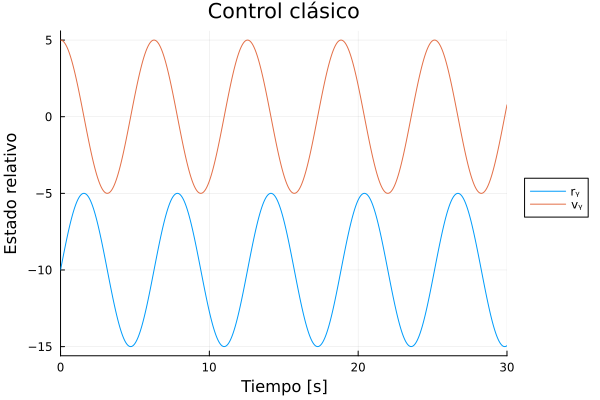
\includegraphics[width=0.76\linewidth]{lineal/estado_control_clasico.png}
  \caption{Chequeo de funcionamiento con el control de prueba $u(t)=5\sin(t)$.}
  \label{fig:lineal-prueba}
\end{figure}

\begin{figure}[H]
  \centering
  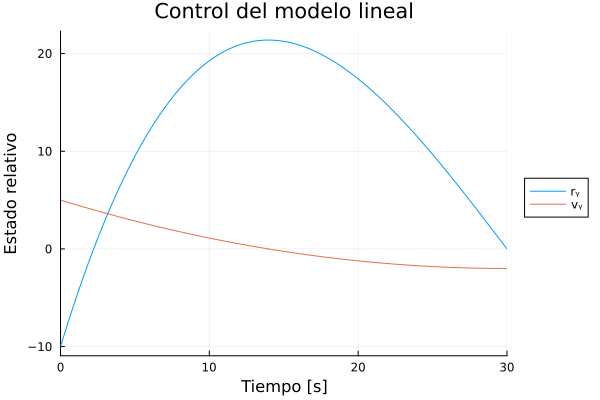
\includegraphics[width=0.76\linewidth]{lineal/estado_control_paper.png}
  \caption{Estado relativo bajo la ley del modelo lineal con restricción dura.}
  \label{fig:lineal-dura}
\end{figure}

\begin{figure}[H]
  \centering
  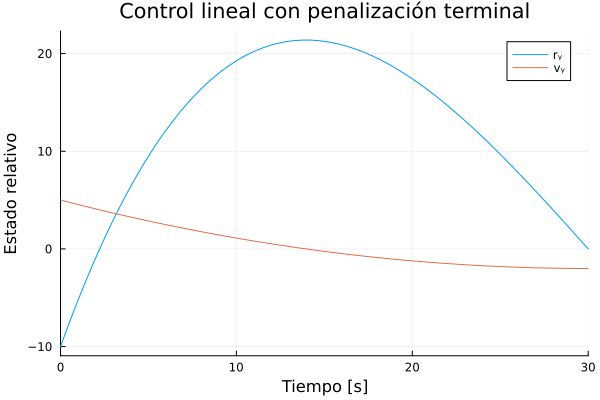
\includegraphics[width=0.76\linewidth]{lineal/estado_control_paper_margen.png}
  \caption{Estado relativo con penalización terminal $q_f=1$.}
  \label{fig:lineal-blanda}
\end{figure}

En las figuras~\ref{fig:lineal-dura} y~\ref{fig:lineal-blanda}, la posición relativa transversal se aproxima a cero al finalizar el intervalo. La velocidad transversal final no es nula. El control de prueba de la figura~\ref{fig:lineal-prueba} produce un comportamiento oscilatorio.

\begin{figure}[H]
  \centering
  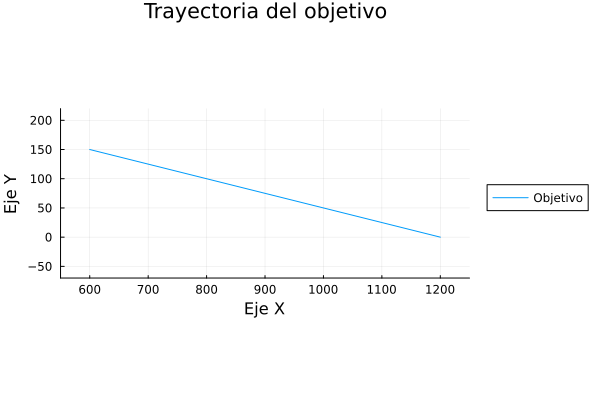
\includegraphics[width=0.76\linewidth]{lineal/trayectoria_objetivo.png}
  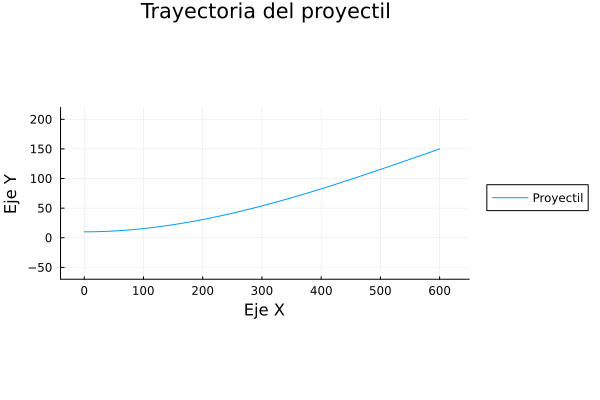
\includegraphics[width=0.76\linewidth]{lineal/trayectoria_proyectil.png}
  \caption{Trayectorias individuales del objetivo y del proyectil.}
  \label{fig:lineal-individuales}
\end{figure}

\begin{figure}[H]
  \centering
  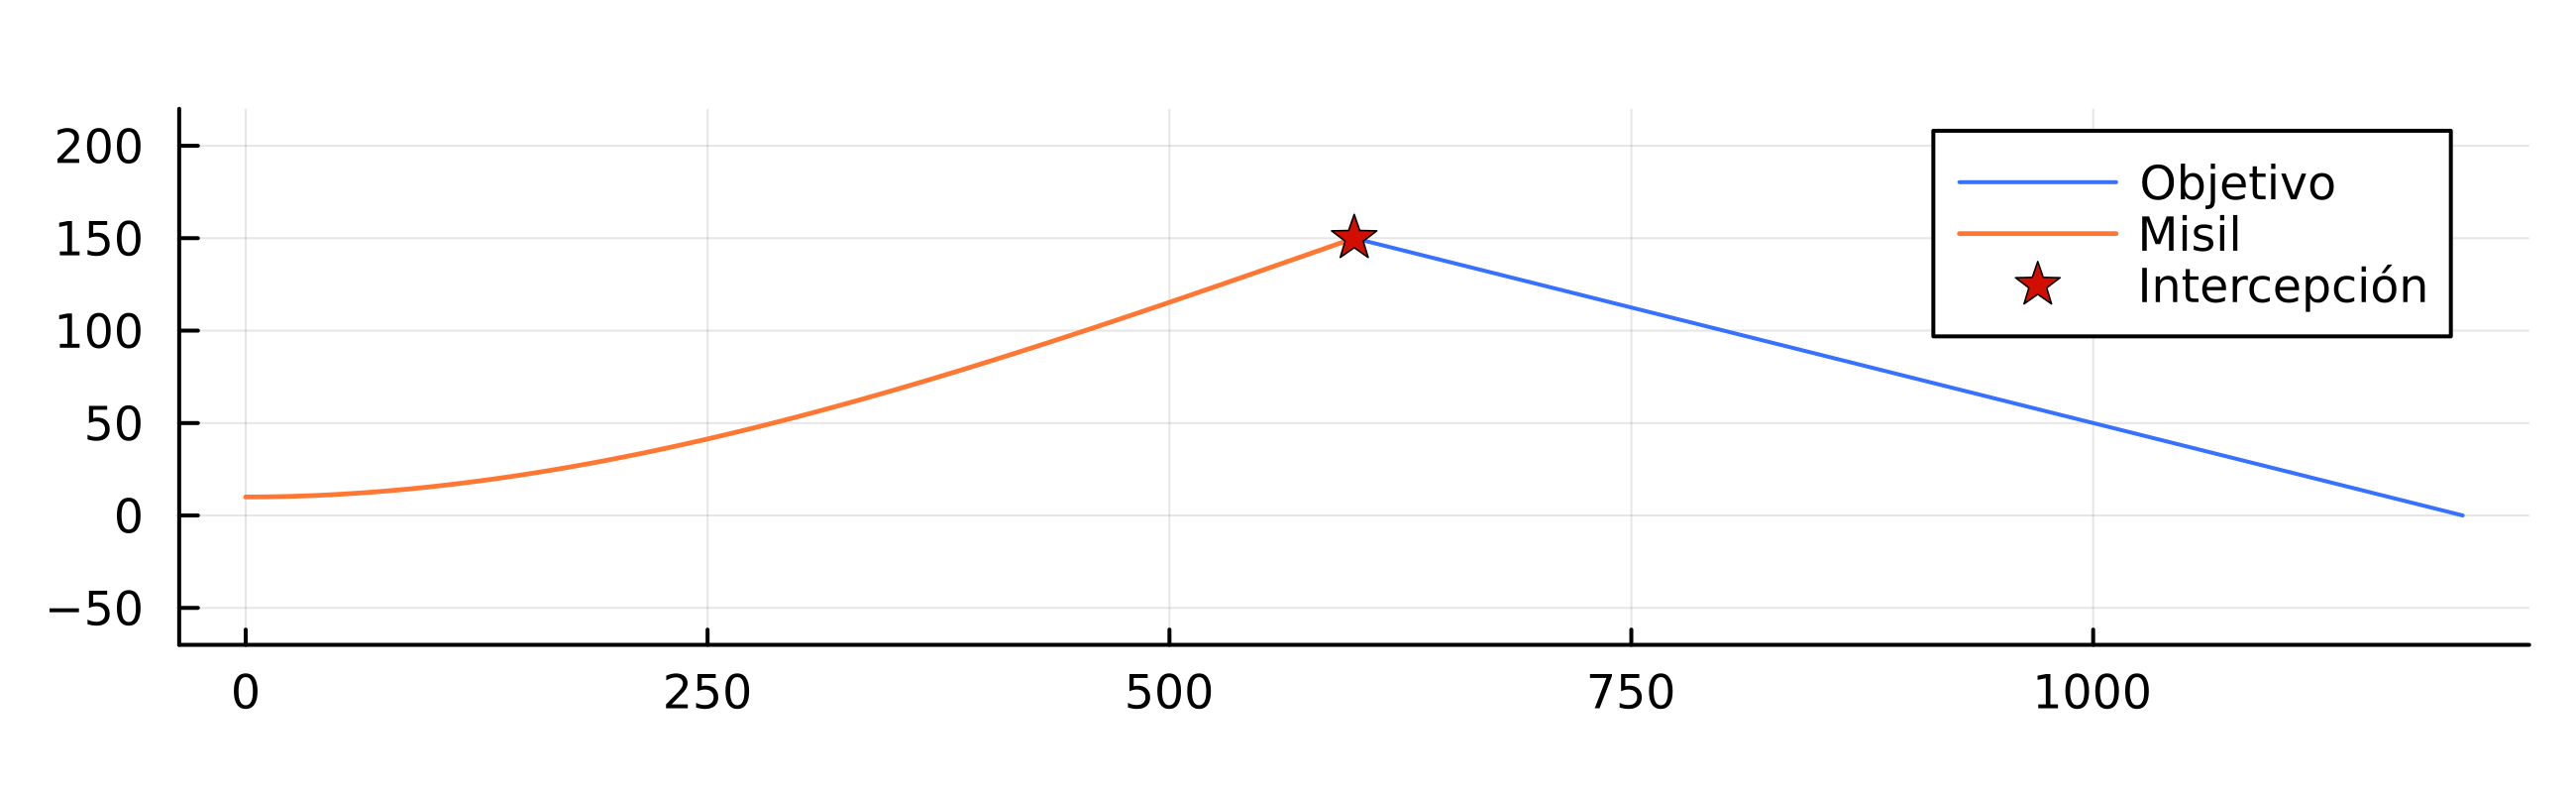
\includegraphics[width=\linewidth]{lineal/colision.png}
  % Leyenda de poster/example.tex.
  \caption{Trayectorias del objetivo y del proyectil bajo control PLC. La estrella indica la intercepción.}
  \label{fig:lineal-colision}
\end{figure}

\begin{figure}[H]
  \centering
  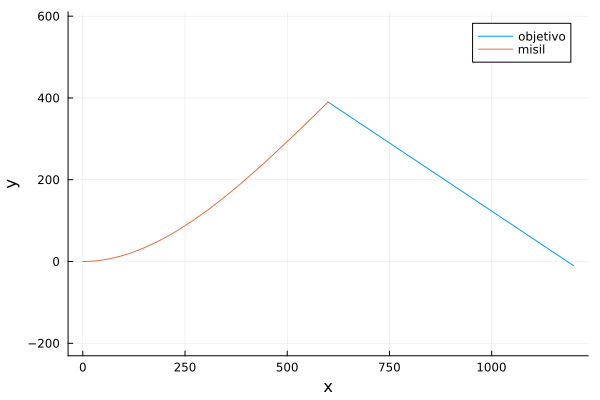
\includegraphics[width=0.76\linewidth]{lineal/lineal_colision.png}
  \caption{Gráfico adicional de trayectorias conservado en \texttt{lineal\_colision.png}. Sus condiciones de simulación no están identificadas en las salidas del notebook actual.}
  \label{fig:lineal-colision-adicional}
\end{figure}

\clearpage
\subsection{Modelo no lineal de un proyectil}
% Fuente: src/modelos/no_lineal.ipynb, celdas 3--13.
Para las simulaciones, asumimos sin pérdida de generalidad que la LOS inicial es paralela al eje $x$, pues en caso contrario basta rotar el sistema.

En \texttt{no\_lineal.ipynb}, el objetivo se ubica en $(60,0)$ y el proyectil parte desde $(0,0)$ con rapidez $V_M=5$. Se consideran los ángulos iniciales $-95^\circ$, $-90^\circ$, $-85^\circ$, $-50^\circ$ y $0^\circ$. Se utilizan $\varepsilon=0.05$, $|u|\leq5$, $t_f\leq20$, \texttt{grid\_size=50} y un máximo de 700 iteraciones. En la implementación, el denominador de la dinámica angular es $\sqrt{r_x^2+r_y^2}+10^{-4}$.

\begin{table}[H]
  \centering
  \caption{Valores registrados por Ipopt en las simulaciones no lineales. $J$ y la violación de restricciones corresponden a los valores sin escalamiento.}
  \label{tab:no-lineal}
  \small
  \begin{tabular}{@{}rrrrrrc@{}}
    \toprule
    $\alpha$ & $\beta$ & $\theta_0$ [$^\circ$] & $J$ & Violación & Iter. & Estado\\
    \midrule
    \filastabla{tablas/no_lineal.tex}
    \bottomrule
  \end{tabular}
\end{table}

Los estados de la tabla~\ref{tab:no-lineal} reproducen los mensajes del solver: O corresponde a \texttt{Optimal Solution Found}, M a \texttt{Maximum Number of Iterations Exceeded} e I a \texttt{Converged to a point of local infeasibility}. Las curvas para $-95^\circ$ y $-90^\circ$ se conservan en los gráficos, pero sus ejecuciones no registran convergencia a una solución factible. Los otros tres ángulos registran el estado O en las tres combinaciones de pesos.

Para $\theta_0=0^\circ$, las tres configuraciones muestran una trayectoria rectilínea. En los casos convergentes con $\theta_0=-85^\circ$ y $-50^\circ$, las trayectorias varían al cambiar los pesos del esfuerzo de control y del tiempo.

\begin{figure}[H]
  \centering
  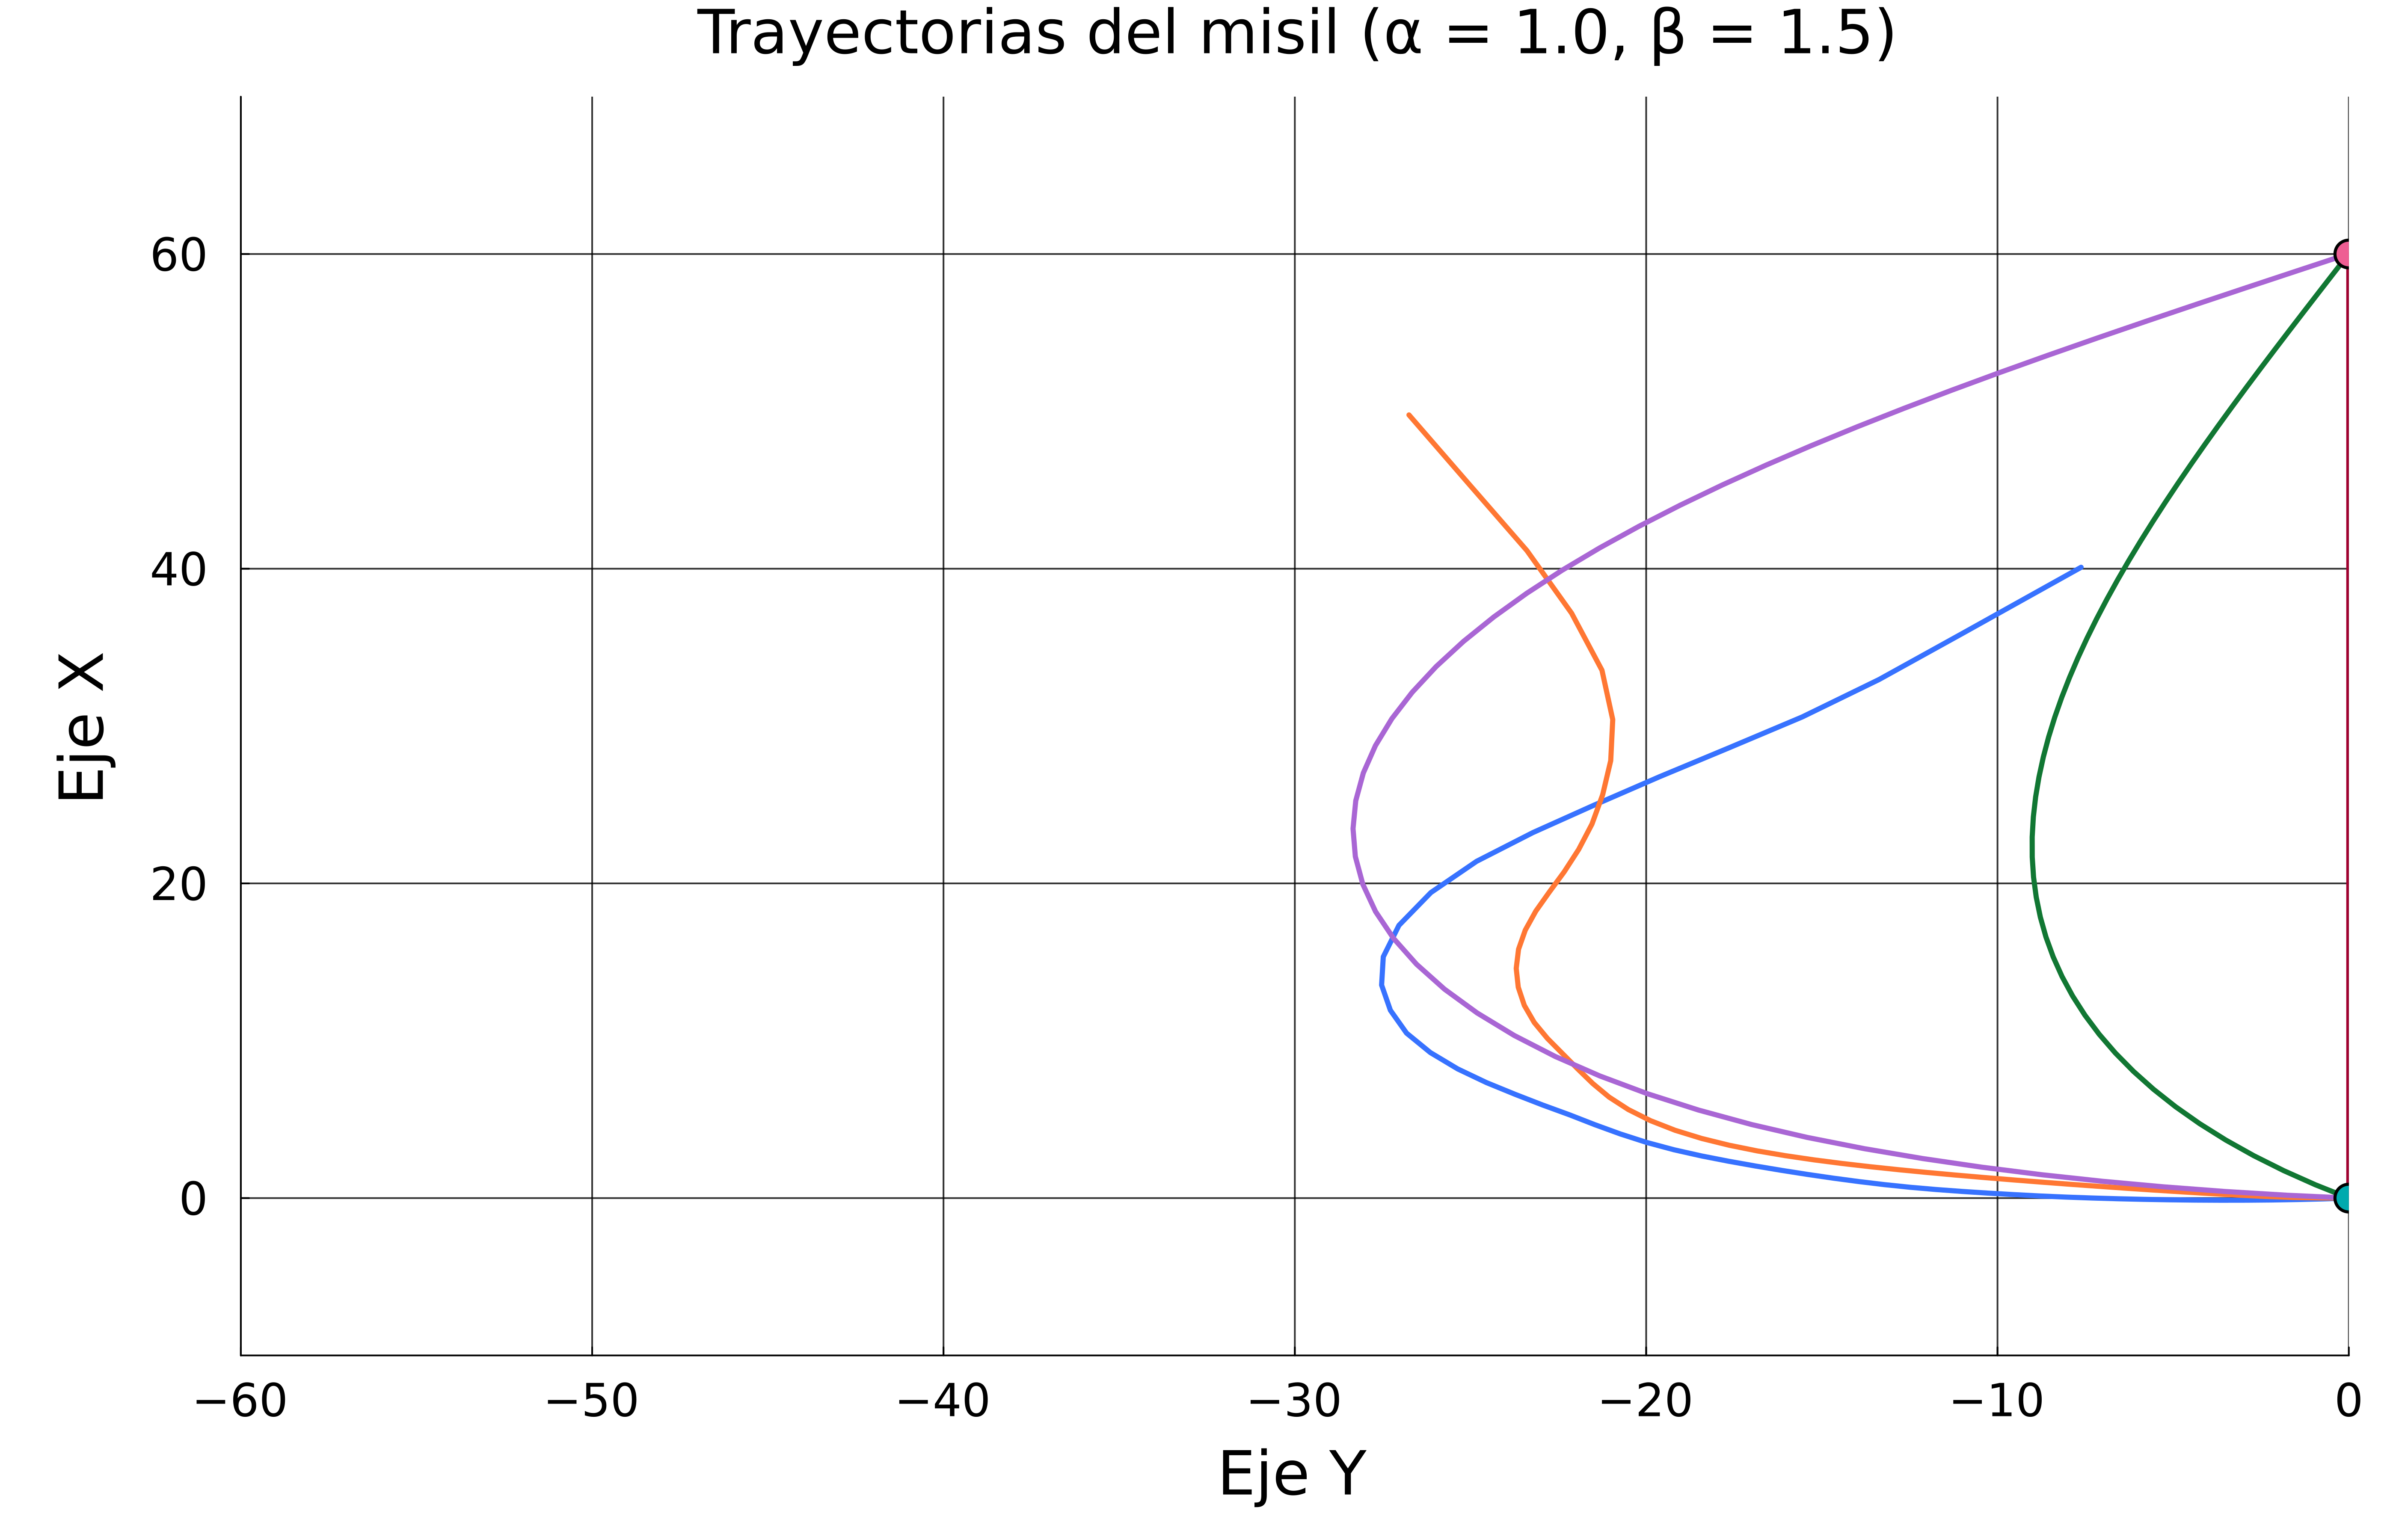
\includegraphics[width=0.9\linewidth]{no_lineal/trayectorias_alpha_1.0_beta_1.5.png}
  \caption{Trayectorias guardadas para $\alpha=1$ y $\beta=1.5$. Los estados de las cinco ejecuciones se indican en la tabla~\ref{tab:no-lineal}.}
  \label{fig:no-lineal-base}
\end{figure}

\begin{figure}[H]
  \centering
  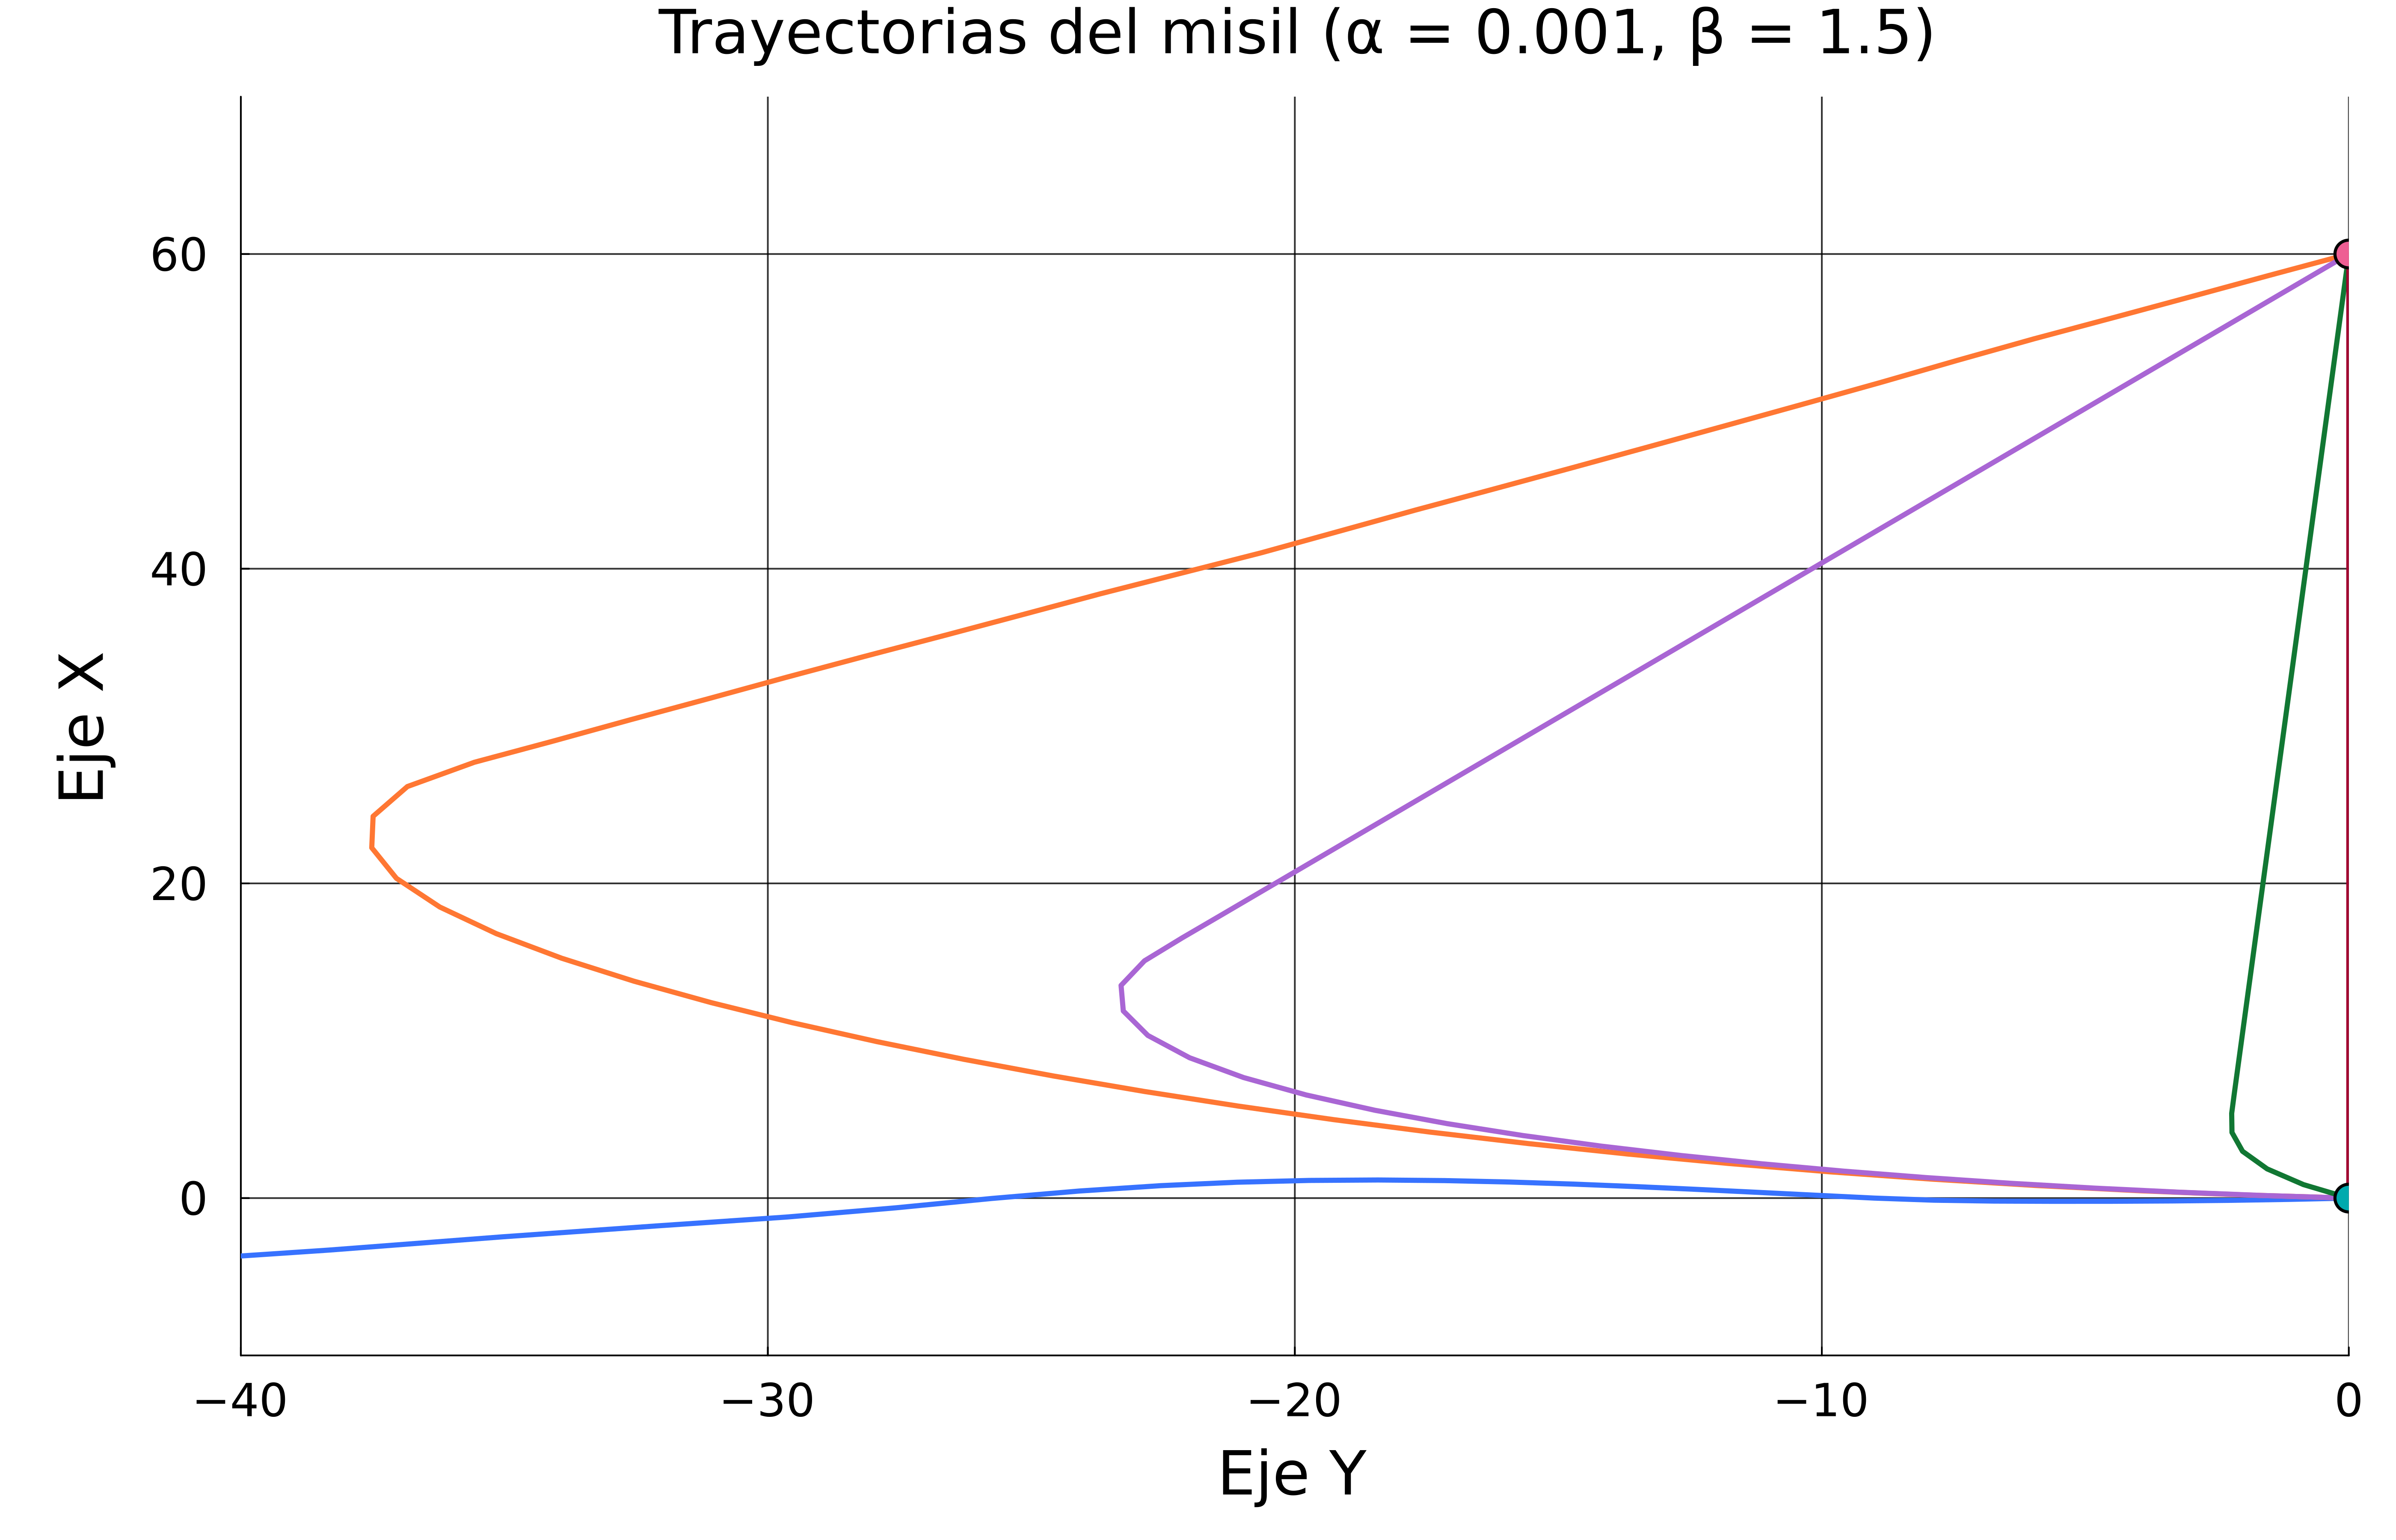
\includegraphics[width=0.9\linewidth]{no_lineal/trayectorias_alpha_0.001_beta_1.5.png}
  \caption{Trayectorias guardadas para $\alpha=0.001$ y $\beta=1.5$.}
  \label{fig:no-lineal-alpha}
\end{figure}

\begin{figure}[H]
  \centering
  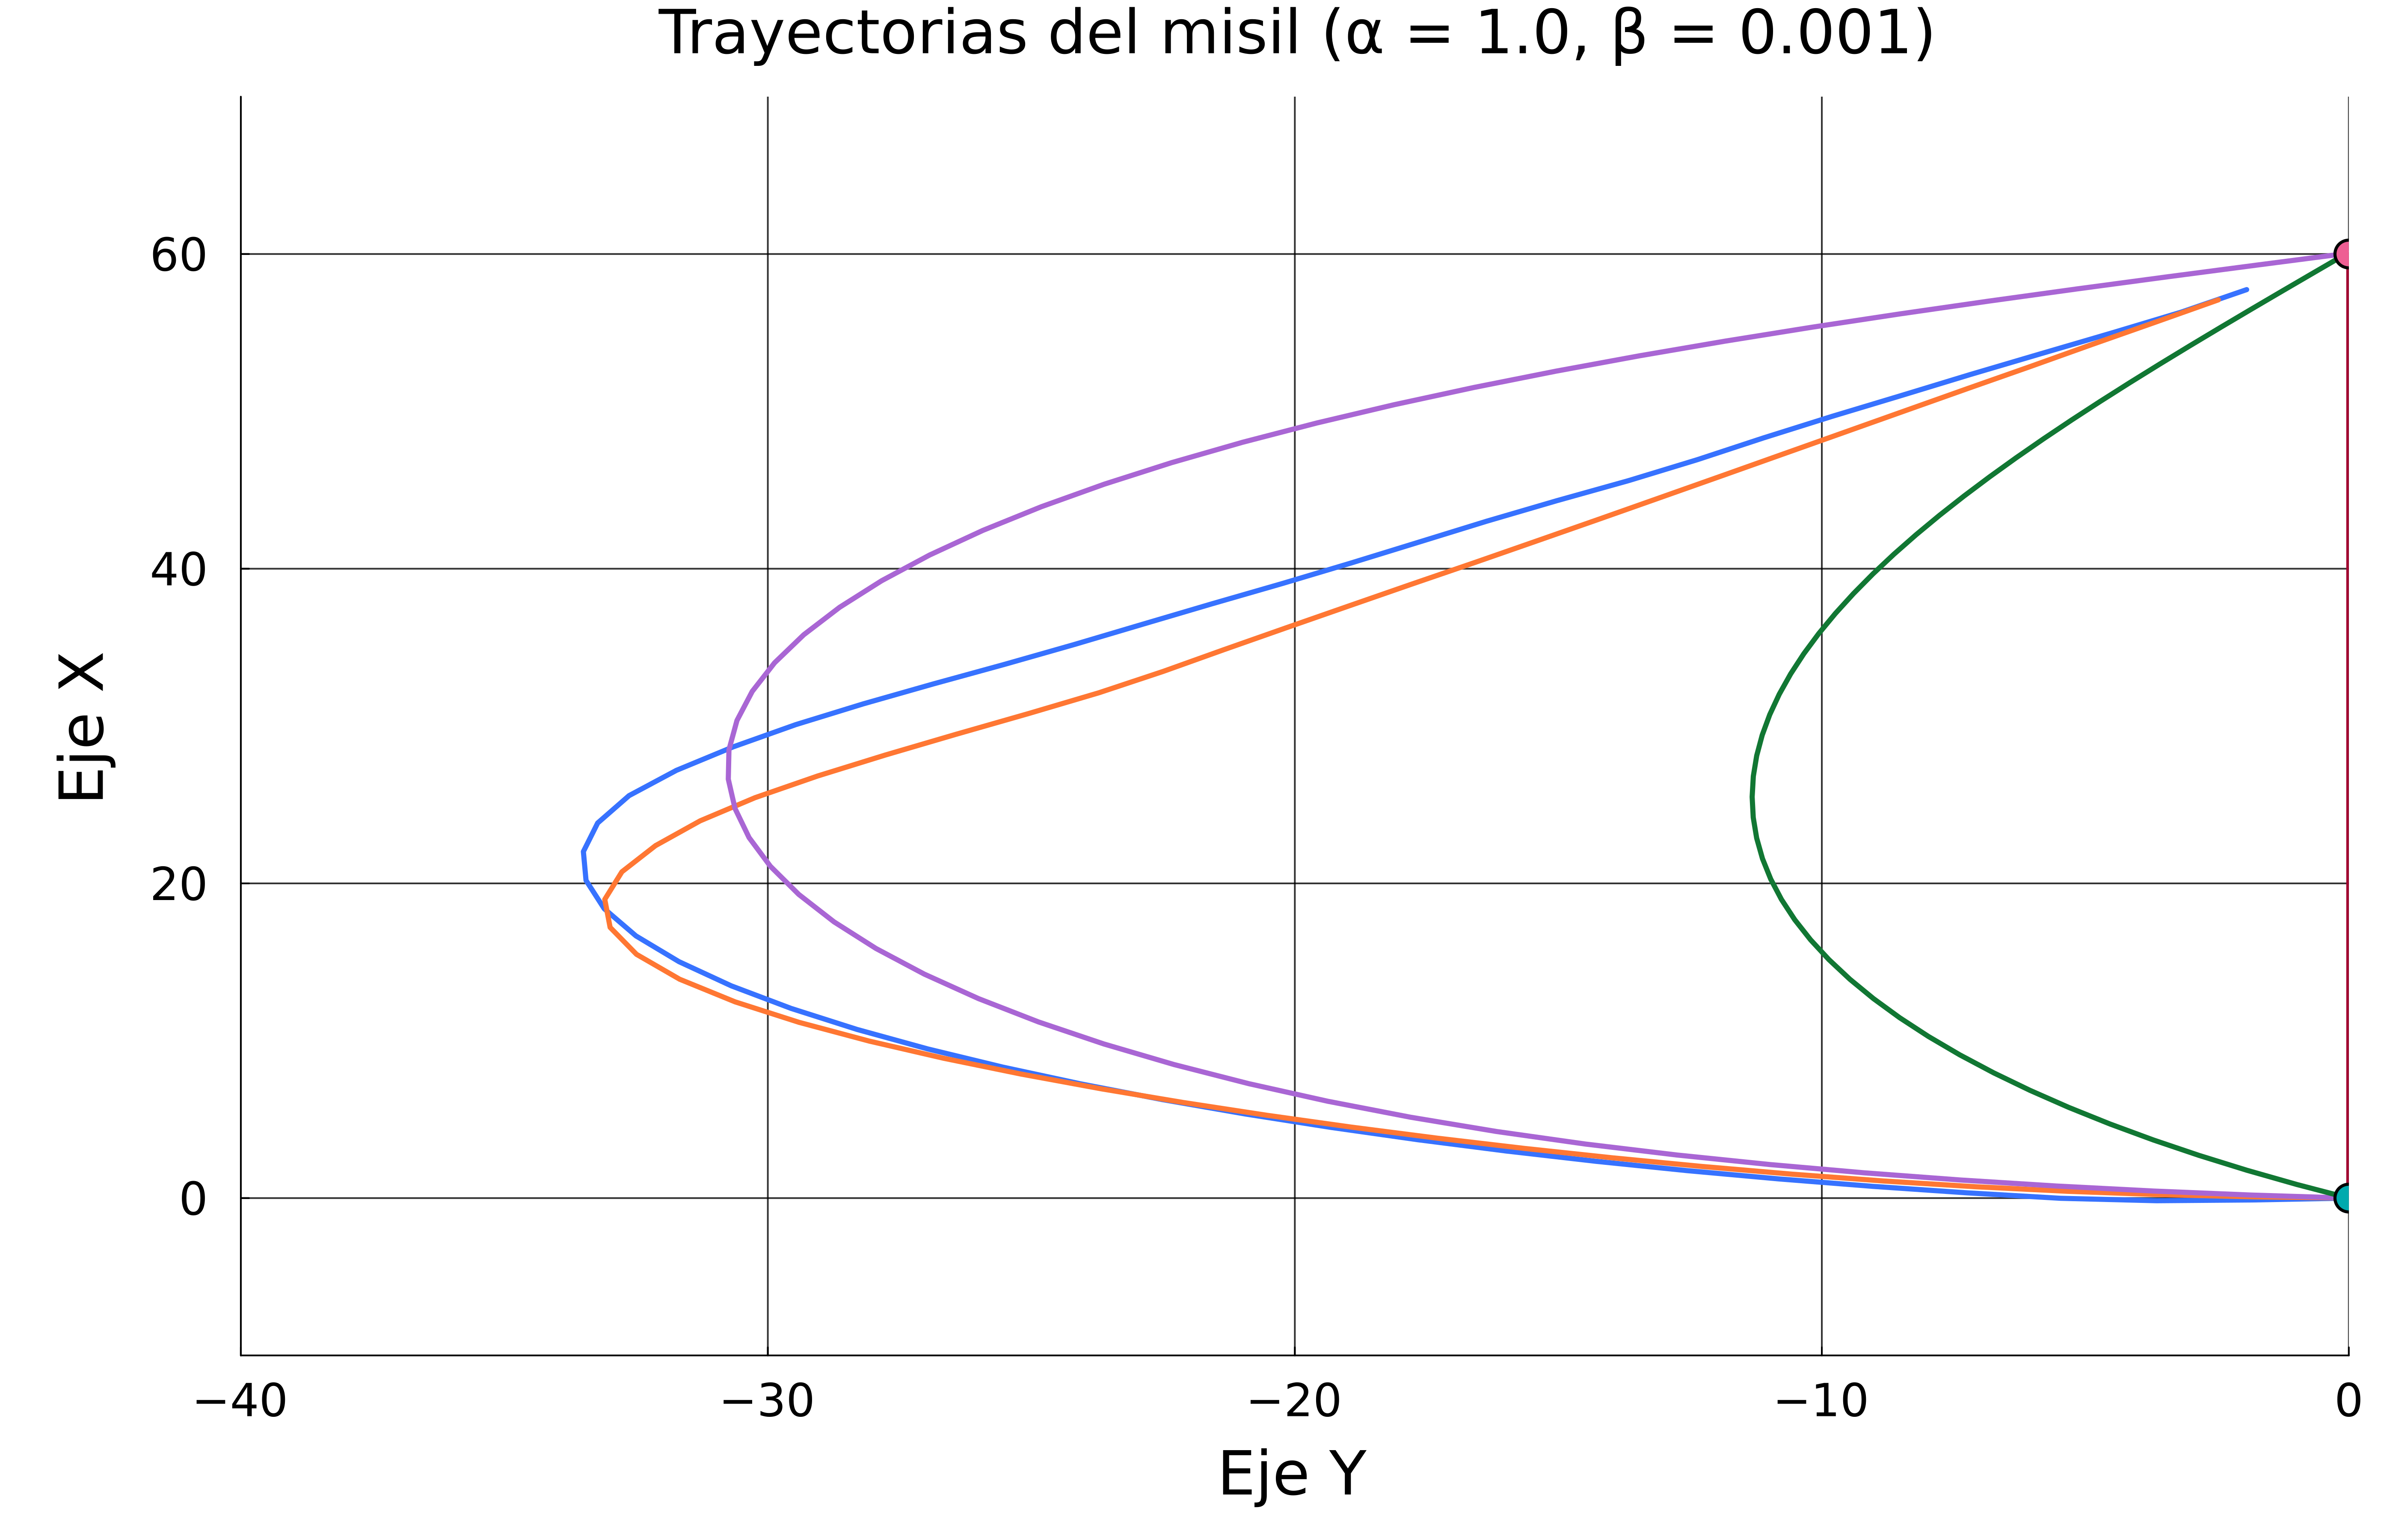
\includegraphics[width=0.9\linewidth]{no_lineal/trayectorias_alpha_1.0_beta_0.001.png}
  \caption{Trayectorias guardadas para $\alpha=1$ y $\beta=0.001$. En las tres figuras individuales, azul corresponde a $-95^\circ$, naranja a $-90^\circ$, violeta a $-85^\circ$, verde a $-50^\circ$ y rojo a $0^\circ$.}
  \label{fig:no-lineal-beta}
\end{figure}

\begin{figure}[H]
  \centering
  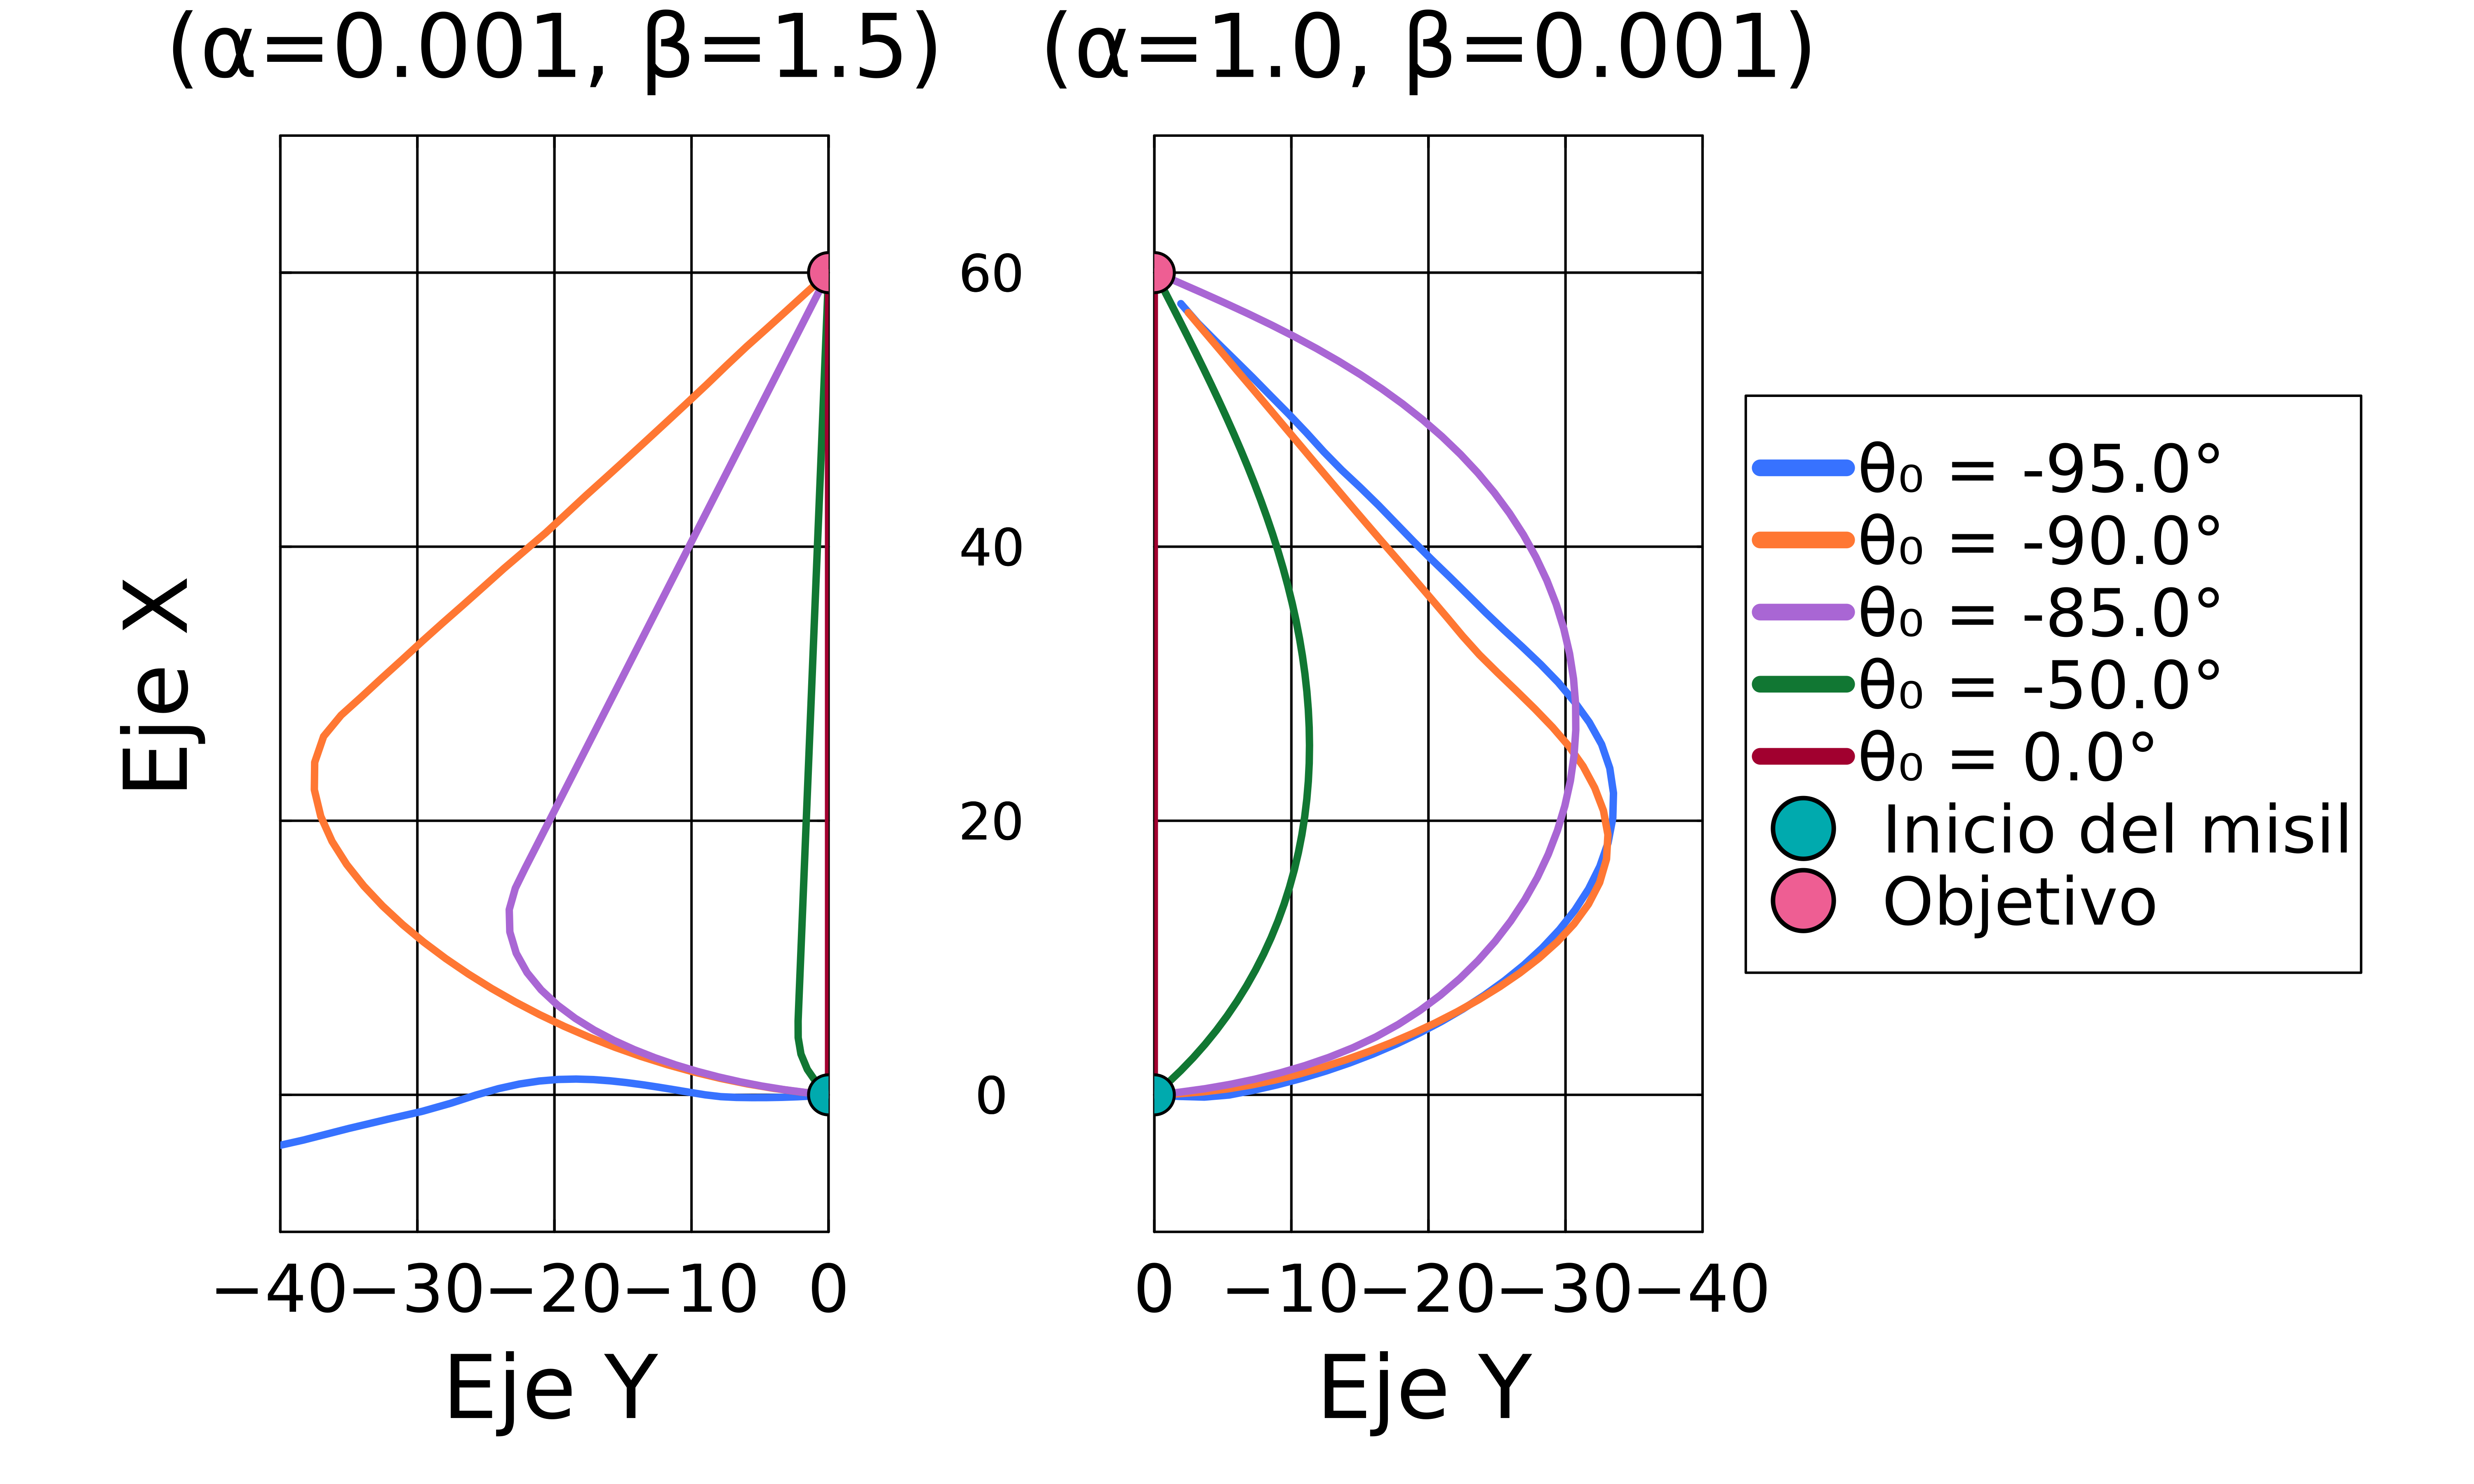
\includegraphics[width=\linewidth]{no_lineal/comparacion.png}
  % Leyenda de poster/example.tex, con los estados documentados en la tabla.
  \caption{Soluciones numéricas comparadas para distintos ángulos iniciales (panel derecho reflejado). Las curvas azul y naranja corresponden a ejecuciones sin convergencia a una solución factible.}
  \label{fig:no-lineal-comparacion}
\end{figure}

\clearpage
\subsection{Dos proyectiles acoplados}
% Fuente: src/modelos/lineal_dos_proyectiles.ipynb, celdas 3--9.
En \texttt{lineal\_dos\_proyectiles.ipynb} se comparan la simulación de la ley analítica y la discretización directa con \texttt{grid\_size=200}. Para el primer experimento se usan
$$
V_M=300,\quad t_f=10,\quad x_0=(200,-10,-250,15),\quad
\theta_d=30^\circ,\quad b=10,\quad c=100.
$$
La resolución numérica registra \texttt{Optimal Solution Found}. El costo sin escalamiento es $4514.4748191008266$ y la violación de restricciones es $2.8421709430404007\times10^{-14}$.

\begin{figure}[H]
  \centering
  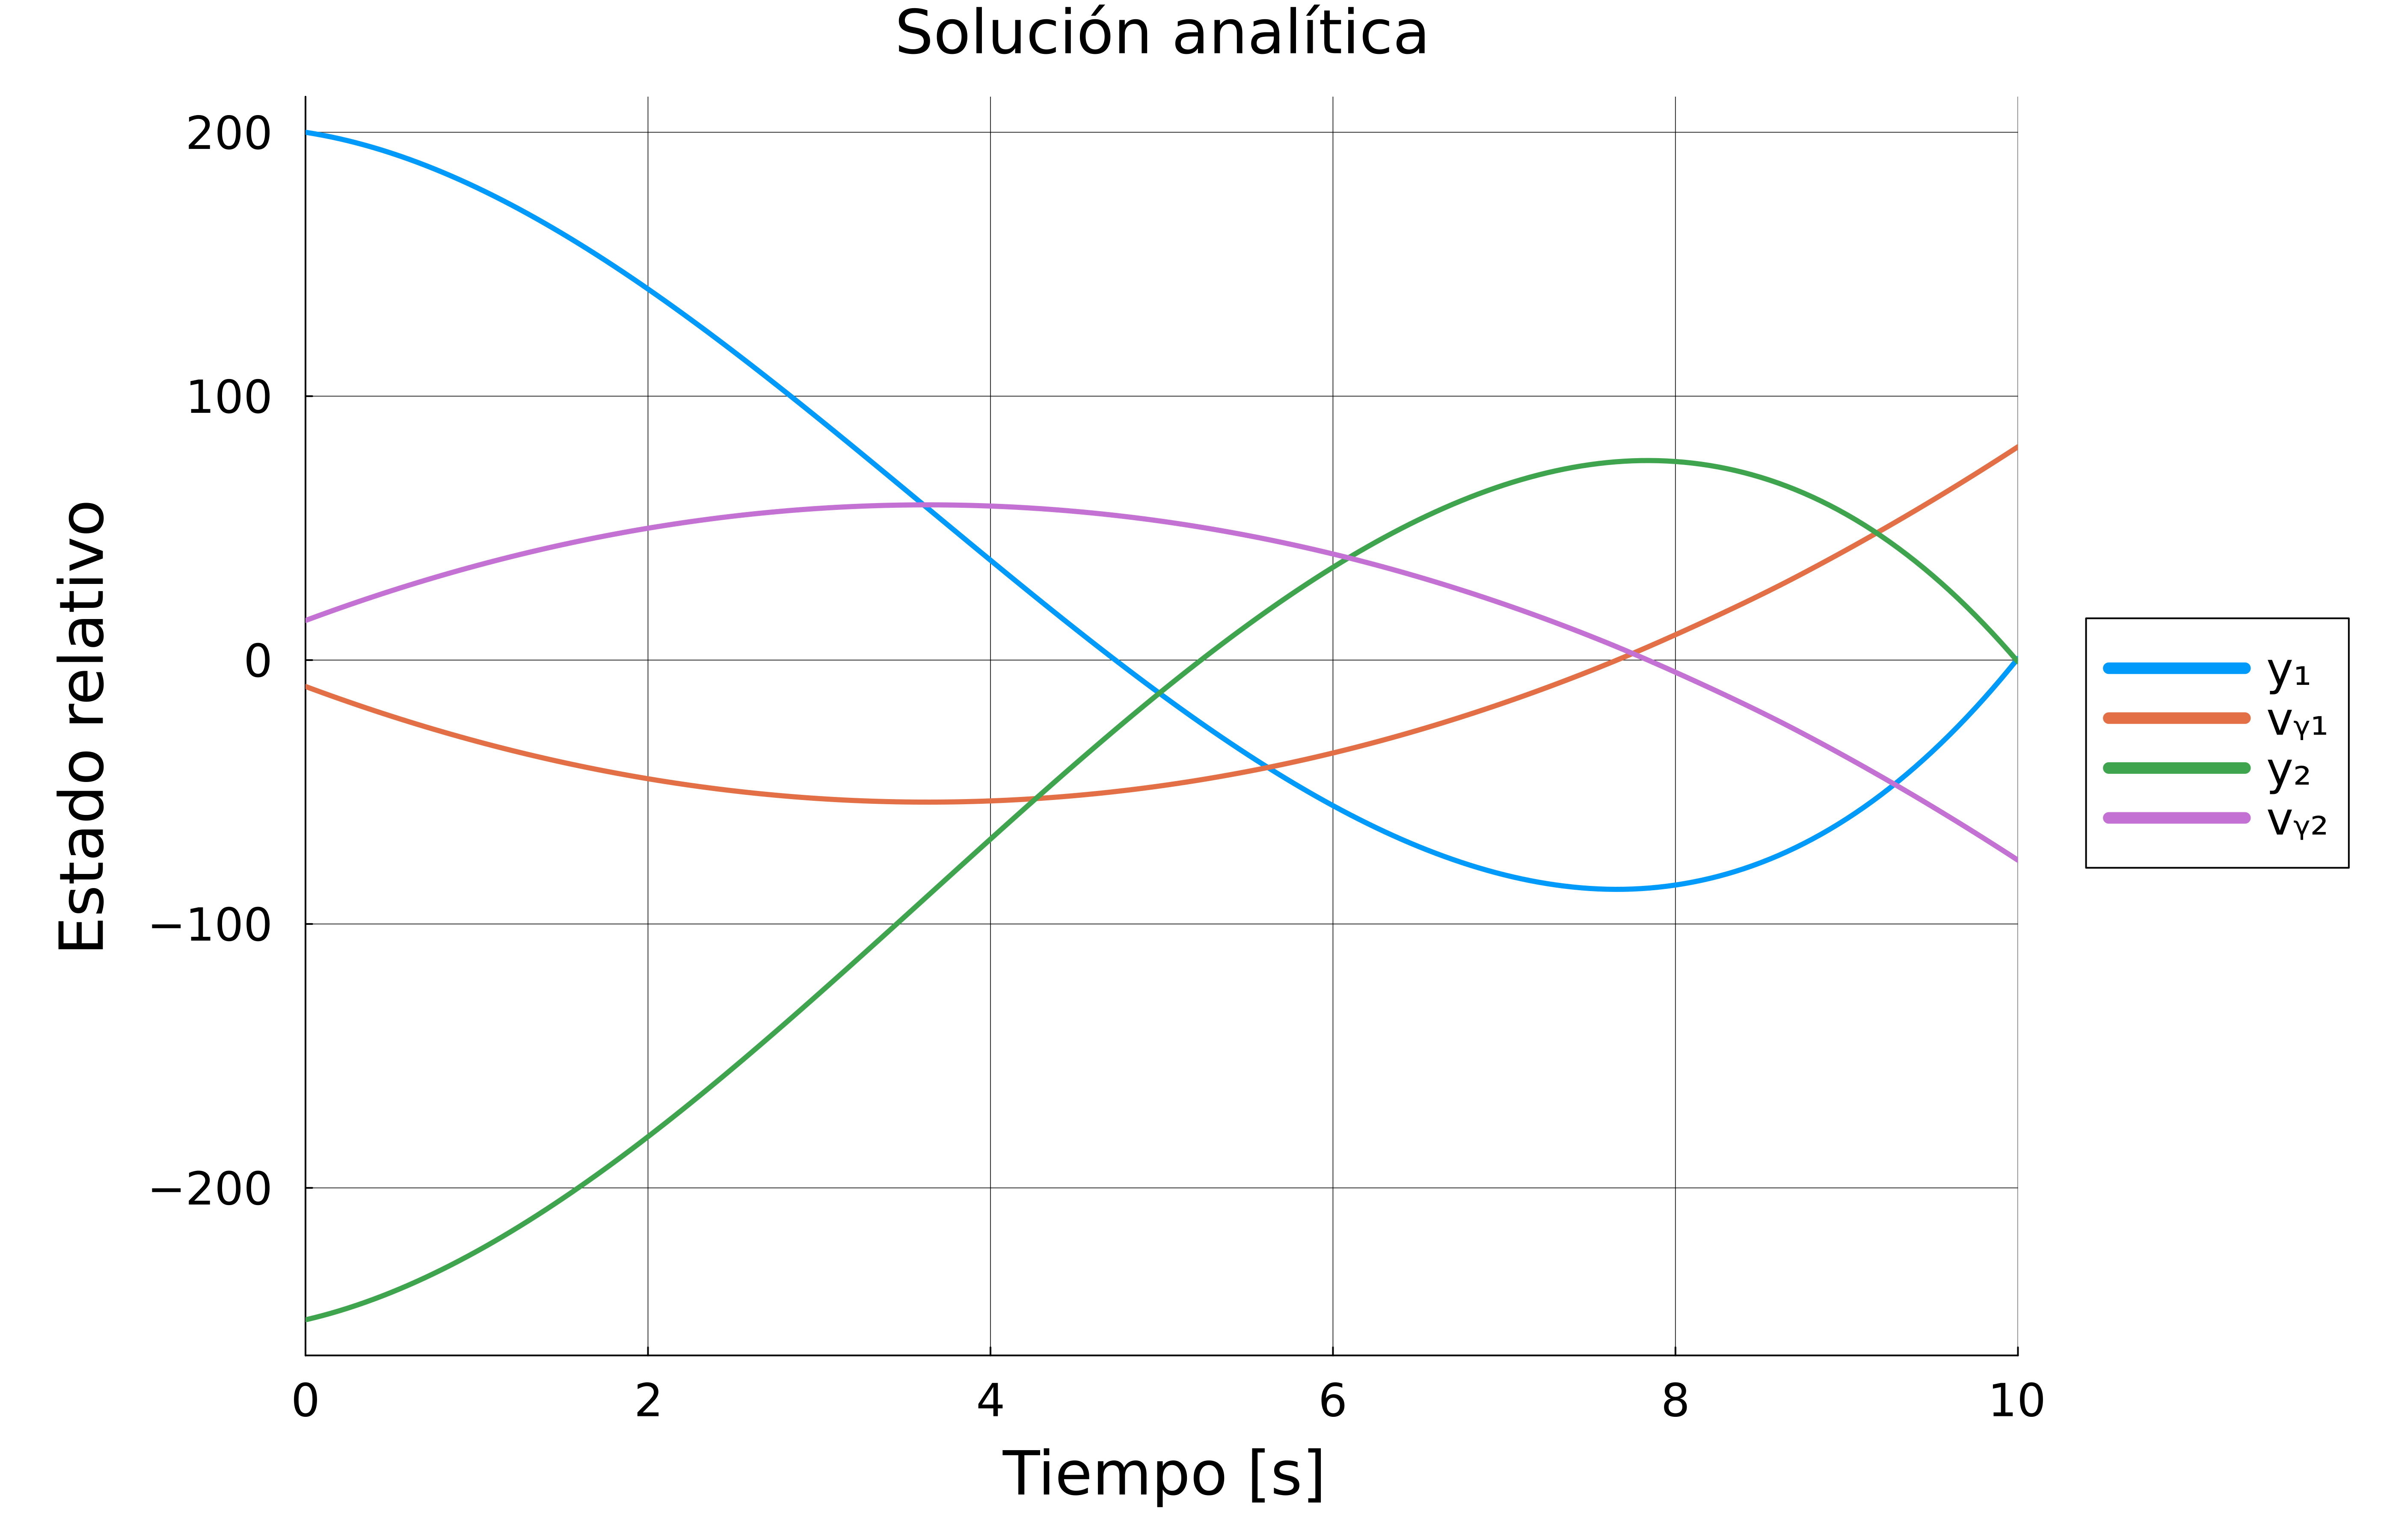
\includegraphics[width=0.95\linewidth]{lineal_dos_proyectiles/solucion_analitica.png}
  \caption{Evolución del estado bajo la ley analítica en el experimento con $\theta_d=30^\circ$.}
  \label{fig:dos-analitica}
\end{figure}

\begin{figure}[H]
  \centering
  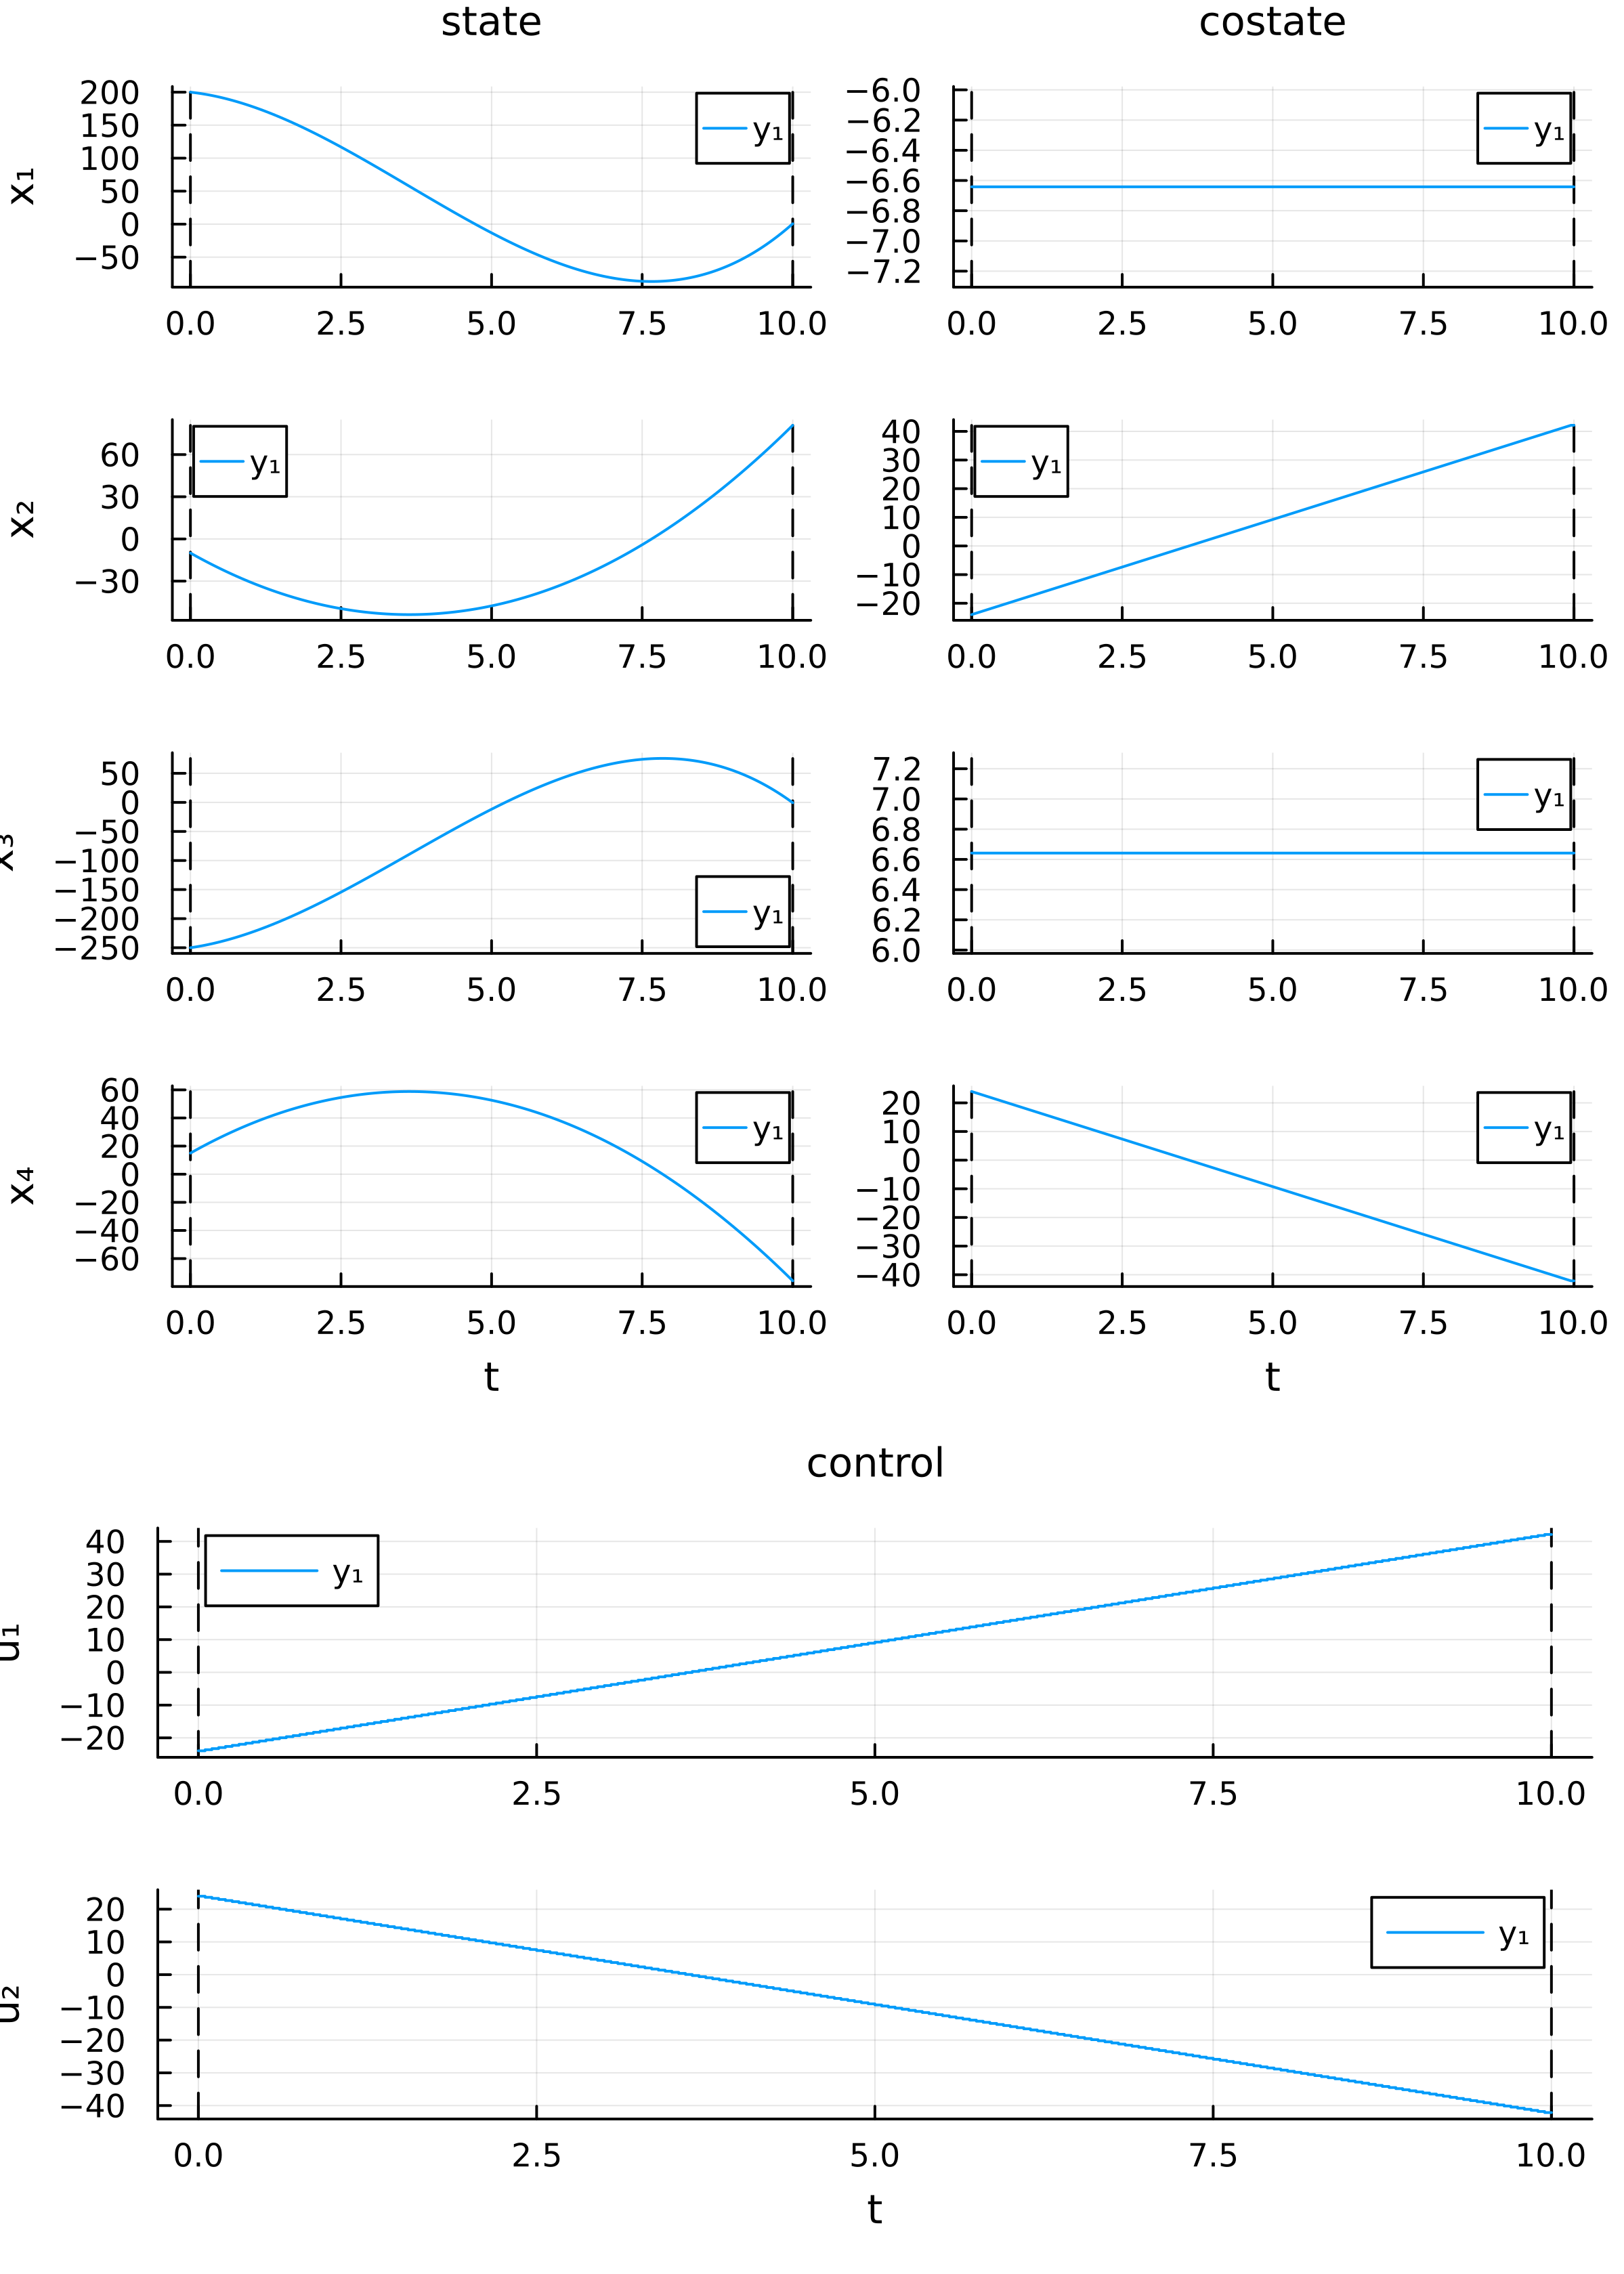
\includegraphics[width=0.93\linewidth,height=0.85\textheight,keepaspectratio]{lineal_dos_proyectiles/solucion_numerica.png}
  \caption{Estados, coestados y controles de la solución numérica para el mismo experimento.}
  \label{fig:dos-numerica}
\end{figure}

Para comparar distintos ángulos relativos de llegada, los proyectiles parten desde $(0,200)$ y $(0,-200)$, con orientación inicial $0^\circ$, y el objetivo se ubica en $(10000,200)$. Se utilizan $V_M=300$, $t_f=10000/300$, $b=1000$ y $c=10$.

\begin{table}[H]
  \centering
  \caption{Ángulos de llegada registrados en el notebook, en grados. La última columna reproduce la diferencia entre $\theta_d$ y $\Delta\theta$ de la solución analítica.}
  \label{tab:angulos}
  \small
  \begin{tabular}{@{}rrrrrrrr@{}}
    \toprule
    & \multicolumn{3}{c}{Analítica} & \multicolumn{3}{c}{Numérica} & Diferencia\\
    \cmidrule(lr){2-4}\cmidrule(lr){5-7}
    $\theta_d$ & $\theta_1$ & $\theta_2$ & $\Delta\theta$ & $\theta_1$ & $\theta_2$ & $\Delta\theta$ & $\theta_d-\Delta\theta$\\
    \midrule
    \filastabla{tablas/angulos.tex}
    \bottomrule
  \end{tabular}
\end{table}

% Texto de poster/example.tex.
Al estar asumiendo el \textbf{modelo lineal} para la obtención del control óptimo, la aproximación angular pierde precisión al aumentar $\theta_d$.
En los valores guardados, la diferencia respecto del ángulo deseado aumenta de $0.2^\circ$ a $45.1^\circ$. Las diferencias angulares obtenidas por los dos métodos son próximas entre sí.

\begin{table}[H]
  \centering
  \caption{Costo y violación de restricciones sin escalamiento en las cuatro resoluciones numéricas. Todas registran \texttt{Optimal Solution Found}.}
  \label{tab:dos-convergencia}
  \begin{tabular}{@{}rrr@{}}
    \toprule
    $\theta_d$ [$^\circ$] & $J$ & Violación de restricciones\\
    \midrule
    \filastabla{tablas/dos_proyectiles.tex}
    \bottomrule
  \end{tabular}
\end{table}

\begin{figure}[H]
  \centering
  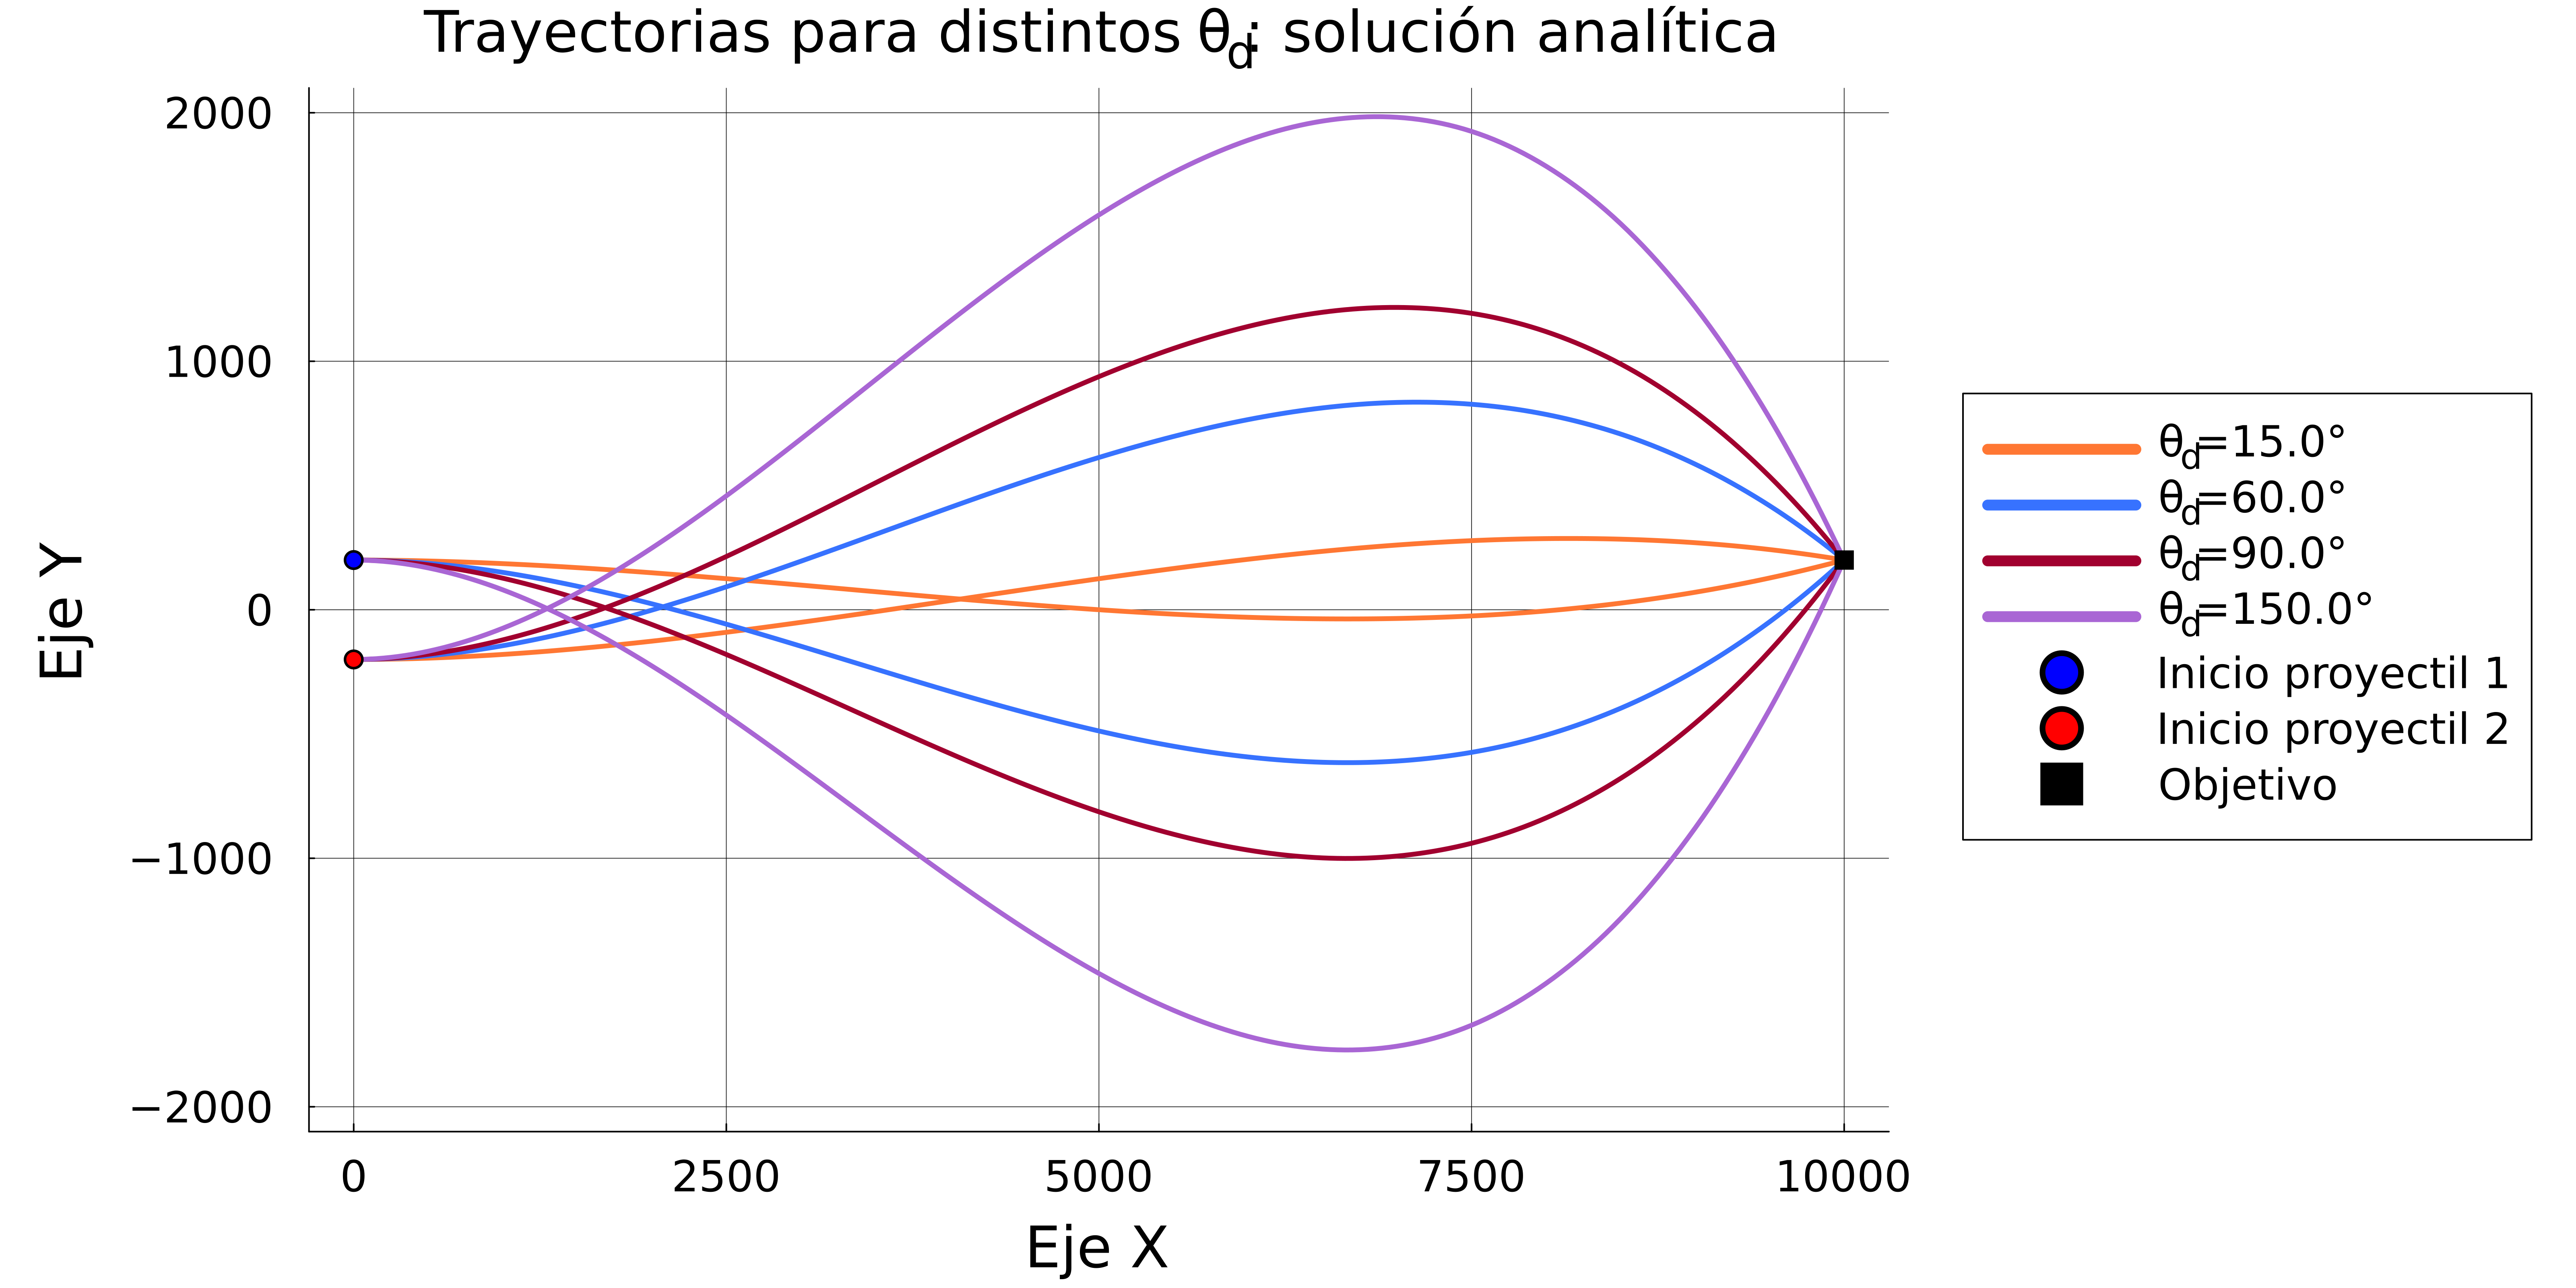
\includegraphics[width=\linewidth]{lineal_dos_proyectiles/comparacion_angulos_analitica.png}
  % Leyenda de poster/example.tex.
  \caption{Trayectorias de la solución analítica para distintos ángulos relativos deseados de llegada.}
  \label{fig:dos-angulos-analitica}
\end{figure}

\begin{figure}[H]
  \centering
  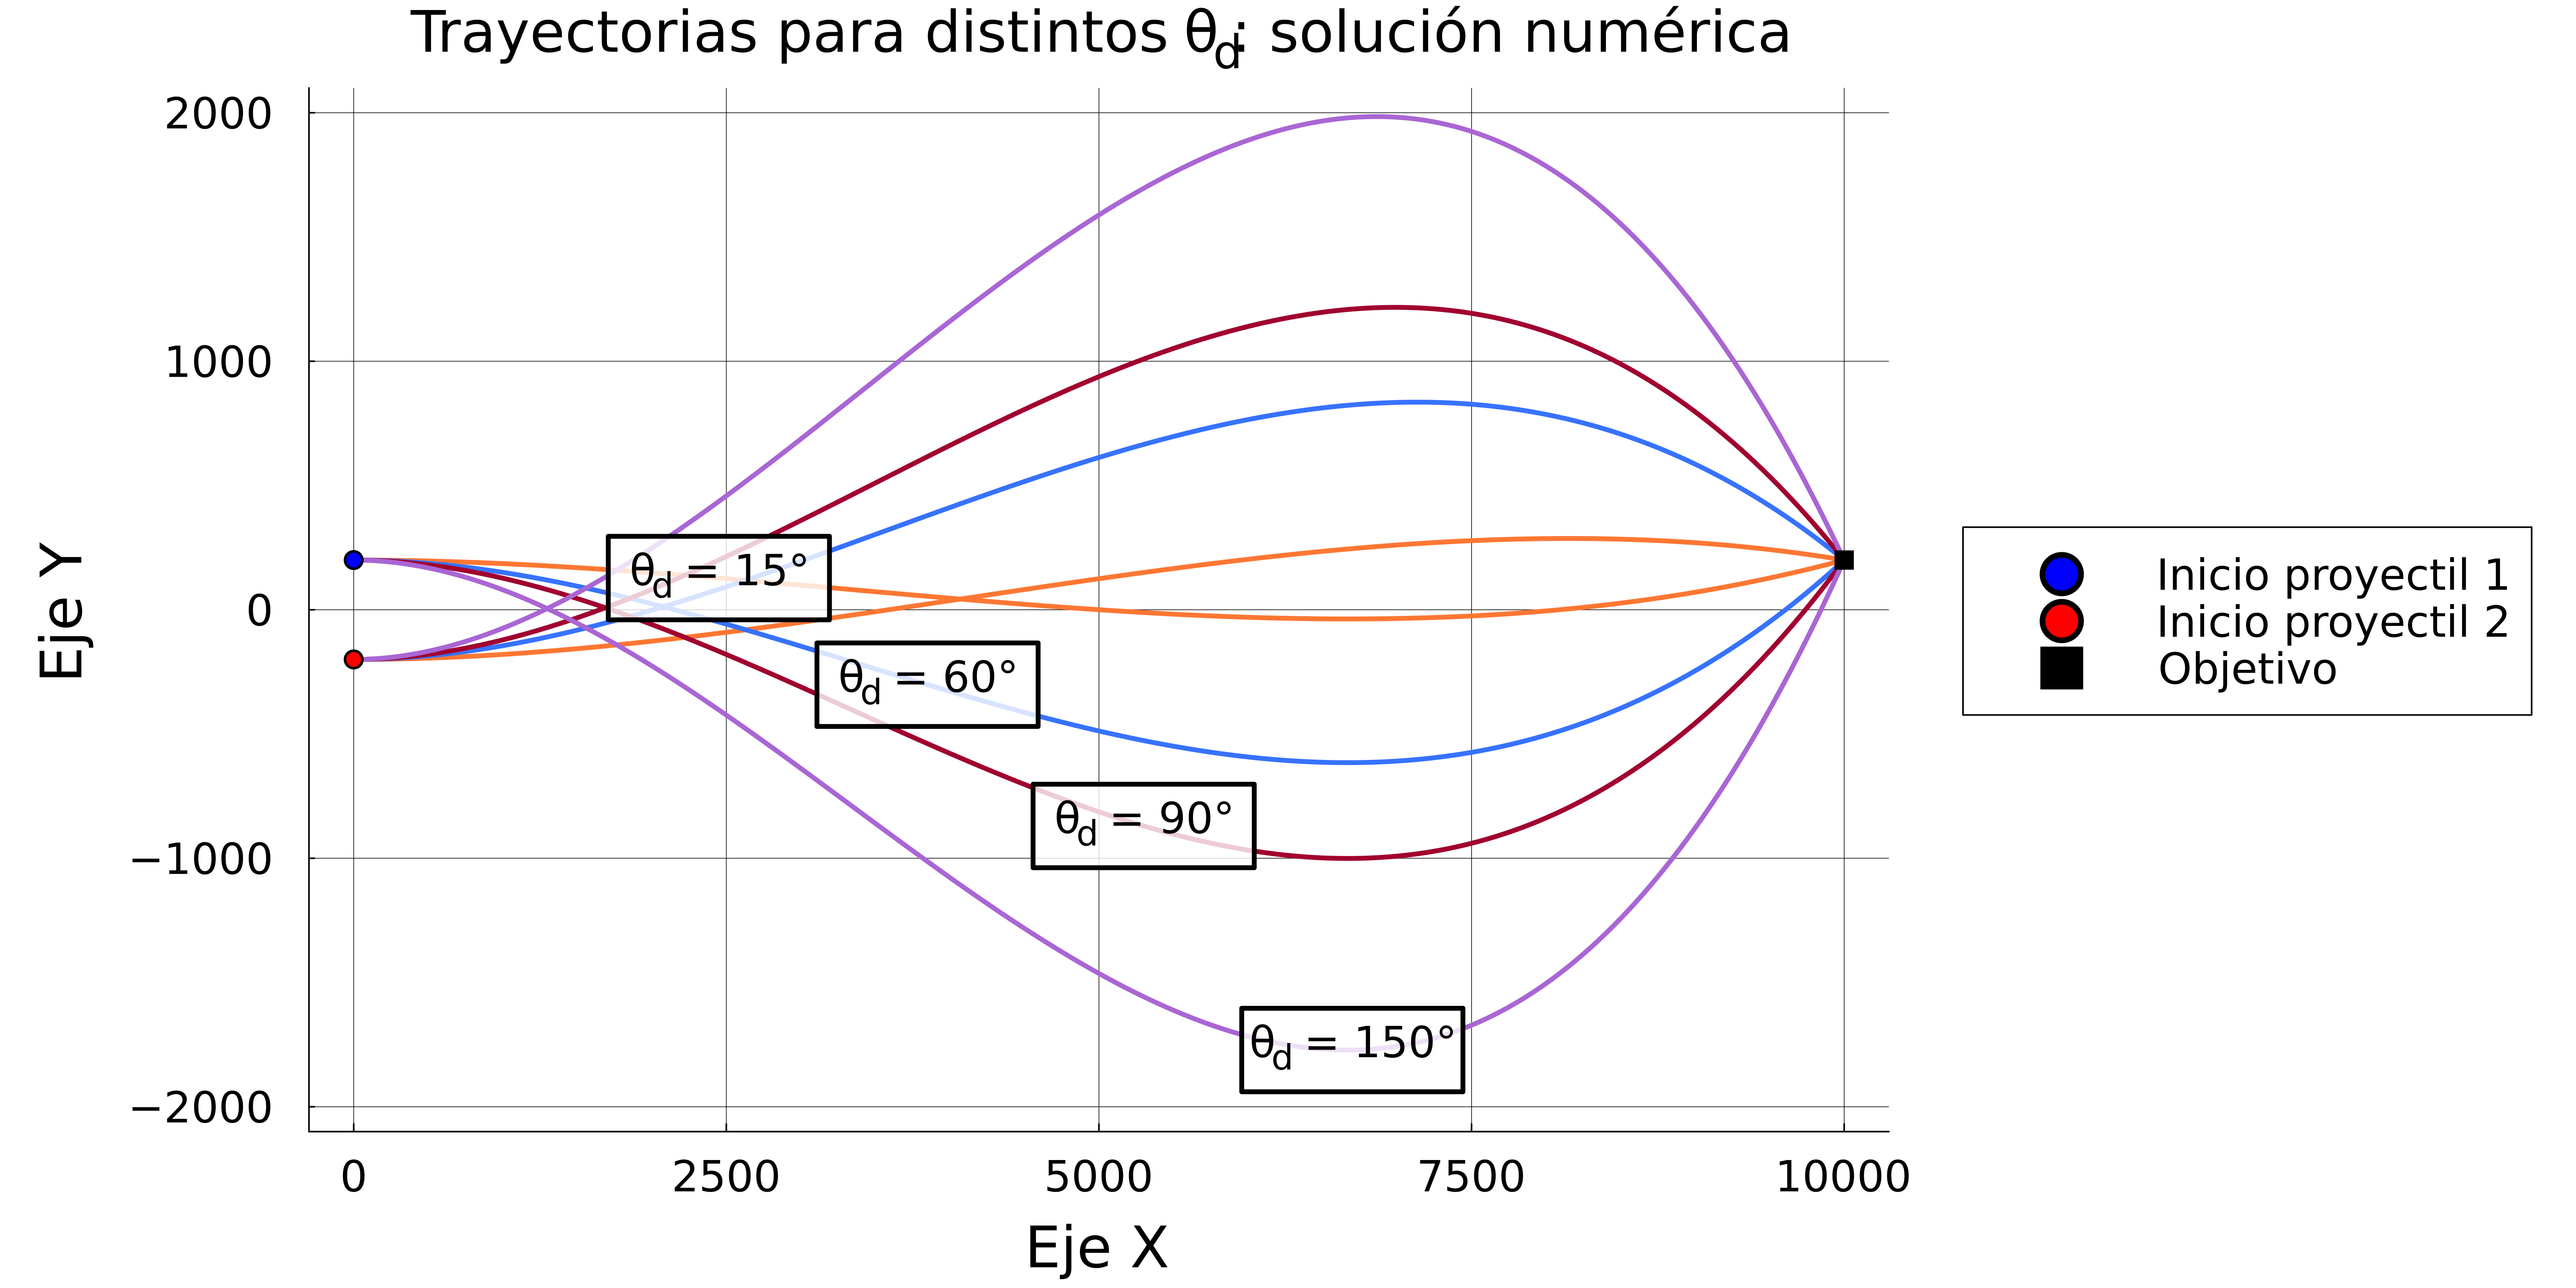
\includegraphics[width=\linewidth]{lineal_dos_proyectiles/comparacion_angulos_numerica.png}
  \caption{Trayectorias de la solución numérica para los mismos ángulos relativos deseados de llegada.}
  \label{fig:dos-angulos-numerica}
\end{figure}

\clearpage
\subsection{Modelo no lineal multiproyectil}
% Fuente: src/modelos/no_lineal_multiproyectil.ipynb, celdas 3, 5 y 9.
Los experimentos de \texttt{no\_lineal\_multiproyectil.ipynb} consideran un objetivo fijo en $(0,0)$ y rapidez $V_M=5$ para todos los proyectiles. Se utilizan $\alpha=1$, $\beta=1.5$, $\gamma=100$, $\varepsilon=0.5$, $|u_i|\leq5$ y un máximo de 6000 iteraciones. Para cada $N$ se toman las primeras $N$ filas de la tabla~\ref{tab:multi-iniciales}. La cota del tiempo final se fija en el código como
$$
t_f\leq\max\left\{35,\ 1.5\cdot1.15\,
\frac{\max_{1\leq i\leq N}\sqrt{r_{x_i}(0)^2+r_{y_i}(0)^2}}{5}\right\}.
$$

\begin{table}[H]
  \centering
  \caption{Posiciones y orientaciones iniciales de los proyectiles.}
  \label{tab:multi-iniciales}
  \begin{tabular}{@{}rrrr@{}}
    \toprule
    $i$ & $x_{M_i}(0)$ & $y_{M_i}(0)$ & $\theta_{M_i}(0)$ [$^\circ$]\\
    \midrule
    1 & 0 & -110 & 100\\
    2 & -110 & -80 & 40\\
    3 & -125 & 10 & 15\\
    4 & -80 & 105 & -40\\
    5 & 10 & 140 & -115\\
    6 & 96 & 72 & -130\\
    7 & 105 & -10 & 160\\
    8 & 75 & -100 & 115\\
    \bottomrule
  \end{tabular}
\end{table}

\begin{table}[H]
  \centering
  \caption{Estado, convergencia y violación de restricciones registrados por \texttt{status}, \texttt{successful} y \texttt{constraints\_violation}.}
  \label{tab:multi-convergencia}
  \begin{tabular}{@{}rllr@{}}
    \toprule
    $N$ & Estado & Convergencia & Violación de restricciones\\
    \midrule
    \filastabla{tablas/multiproyectil.tex}
    \bottomrule
  \end{tabular}
\end{table}

Las ocho ejecuciones registran convergencia. La mayor violación de restricciones reportada corresponde a $N=4$, con aproximadamente $1.15\times10^{-6}$. Estos registros corresponden al problema discretizado. El tiempo final común y la penalización de las holguras no constituyen una comprobación de que todas las primeras llegadas ocurran exactamente al mismo instante.

\begin{figure}[H]
  \centering
  \includegraphics[width=\linewidth]{multiproyectil/trayectorias_N1.png}
  \caption{Trayectoria de un proyectil con penalización de entrada anticipada. \href{run:figuras/multiproyectil/trayectorias_N1.gif}{Animación original}.}
  \label{fig:multi-1}
\end{figure}

\begin{figure}[H]
  \centering
  \includegraphics[width=\linewidth]{multiproyectil/trayectorias_N2.png}
  \caption{Trayectorias de 2 proyectiles con tiempo final común y penalización de llegadas anticipadas.}
  \label{fig:multi-2}
\end{figure}

\begin{figure}[H]
  \centering
  \includegraphics[width=\linewidth]{multiproyectil/trayectorias_N3.png}
  \caption{Trayectorias de 3 proyectiles con tiempo final común y penalización de llegadas anticipadas. \href{run:figuras/multiproyectil/trayectorias_N3.gif}{Animación original}.}
  \label{fig:multi-3}
\end{figure}

\begin{figure}[H]
  \centering
  \includegraphics[width=\linewidth]{multiproyectil/trayectorias_N4.png}
  \caption{Trayectorias de 4 proyectiles con tiempo final común y penalización de llegadas anticipadas. \href{run:figuras/multiproyectil/trayectorias_N4.gif}{Animación original}.}
  \label{fig:multi-4}
\end{figure}

\begin{figure}[H]
  \centering
  \includegraphics[width=\linewidth]{multiproyectil/trayectorias_N5.png}
  \caption{Trayectorias de 5 proyectiles con tiempo final común y penalización de llegadas anticipadas. \href{run:figuras/multiproyectil/trayectorias_N5.gif}{Animación original}.}
  \label{fig:multi-5}
\end{figure}

\begin{figure}[H]
  \centering
  \includegraphics[width=\linewidth]{multiproyectil/trayectorias_N6.png}
  \caption{Trayectorias de 6 proyectiles con tiempo final común y penalización de llegadas anticipadas. \href{run:figuras/multiproyectil/trayectorias_N6.gif}{Animación original}.}
  \label{fig:multi-6}
\end{figure}

\begin{figure}[H]
  \centering
  \includegraphics[width=\linewidth]{multiproyectil/trayectorias_N7.png}
  \caption{Trayectorias de 7 proyectiles con tiempo final común y penalización de llegadas anticipadas. \href{run:figuras/multiproyectil/trayectorias_N7.gif}{Animación original}.}
  \label{fig:multi-7}
\end{figure}

\begin{figure}[H]
  \centering
  \includegraphics[width=\linewidth]{multiproyectil/trayectorias_N8.png}
  \caption{Trayectorias de 8 proyectiles con tiempo final común y penalización de llegadas anticipadas. \href{run:figuras/multiproyectil/trayectorias_N8.gif}{Animación original}.}
  \label{fig:multi-8}
\end{figure}


\subsubsection{Dos proyectiles con distancias iniciales diferentes}
% Fuente: última celda de src/modelos/no_lineal_multiproyectil.ipynb y GIF existentes.
El segundo experimento utiliza posiciones iniciales $(-10,0)$ y $(150,0)$, orientaciones $45^\circ$ y $225^\circ$, rapidez $V_M=2$ y pesos $\gamma=100$ y $\gamma=0.0001$. El código fija $t_f\leq(150/2)\cdot1.15\cdot1.5$. Se conservan las dos animaciones, pero la celda no contiene salidas de estado del solver ni valores de violación de restricciones.

\begin{figure}[H]
  \centering
  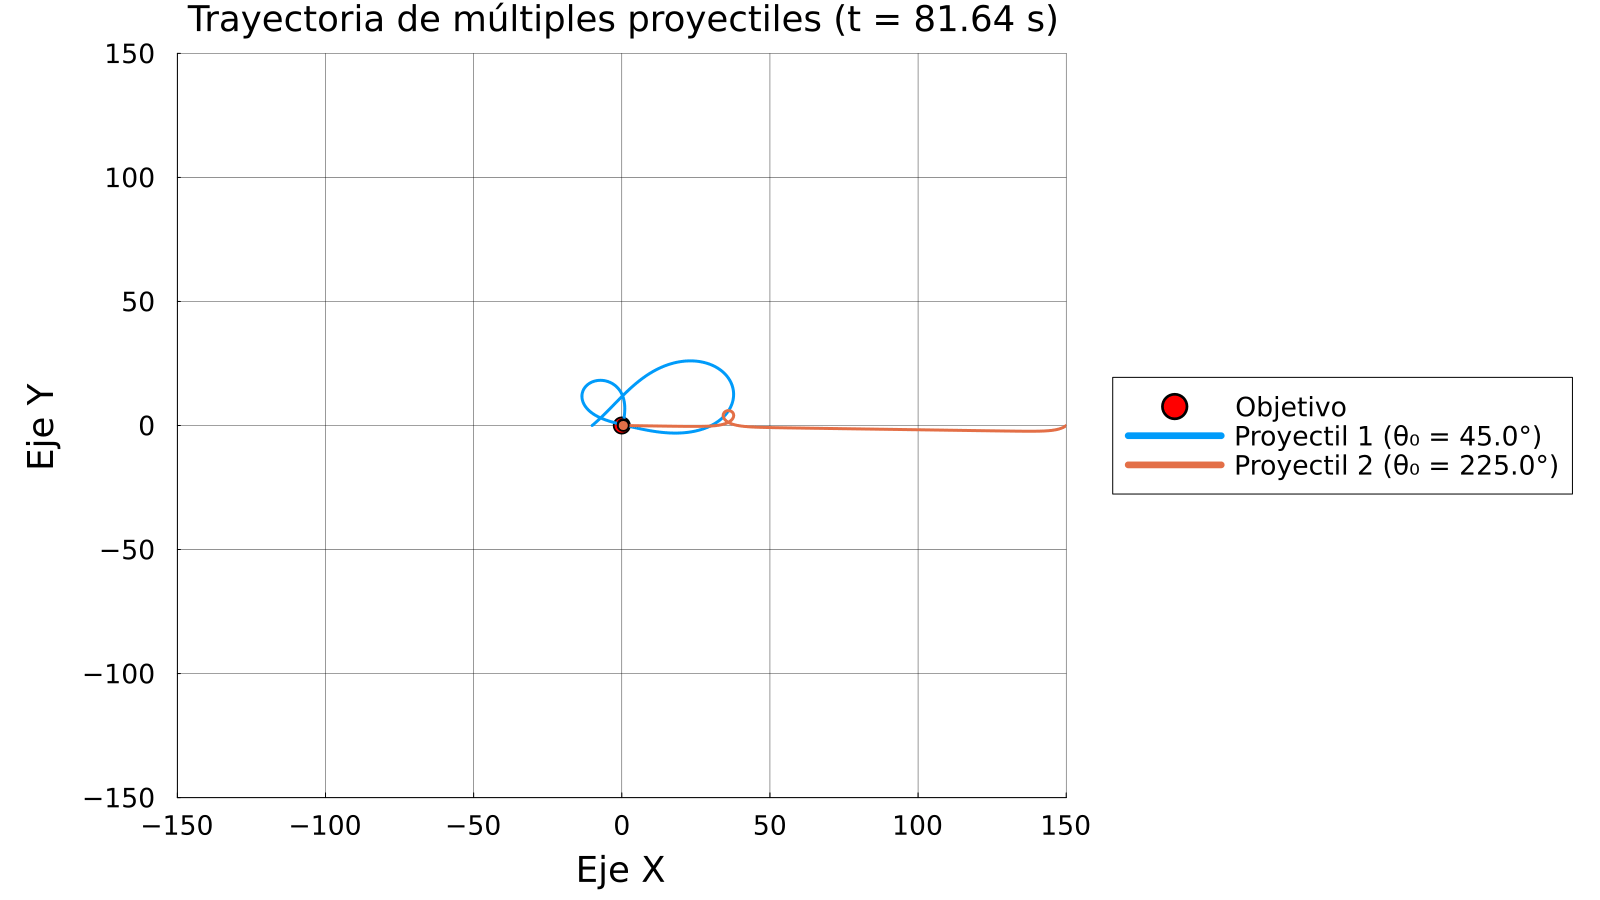
\includegraphics[width=\linewidth]{multiproyectil/posiciones_lejanas_gamma_100.0_final.png}
  \caption{Último fotograma de la animación guardada con $\gamma=100$. \href{run:figuras/multiproyectil/posiciones_lejanas_gamma_100.0.gif}{Animación original}.}
  \label{fig:multi-lejanas-alta}
\end{figure}

\begin{figure}[H]
  \centering
  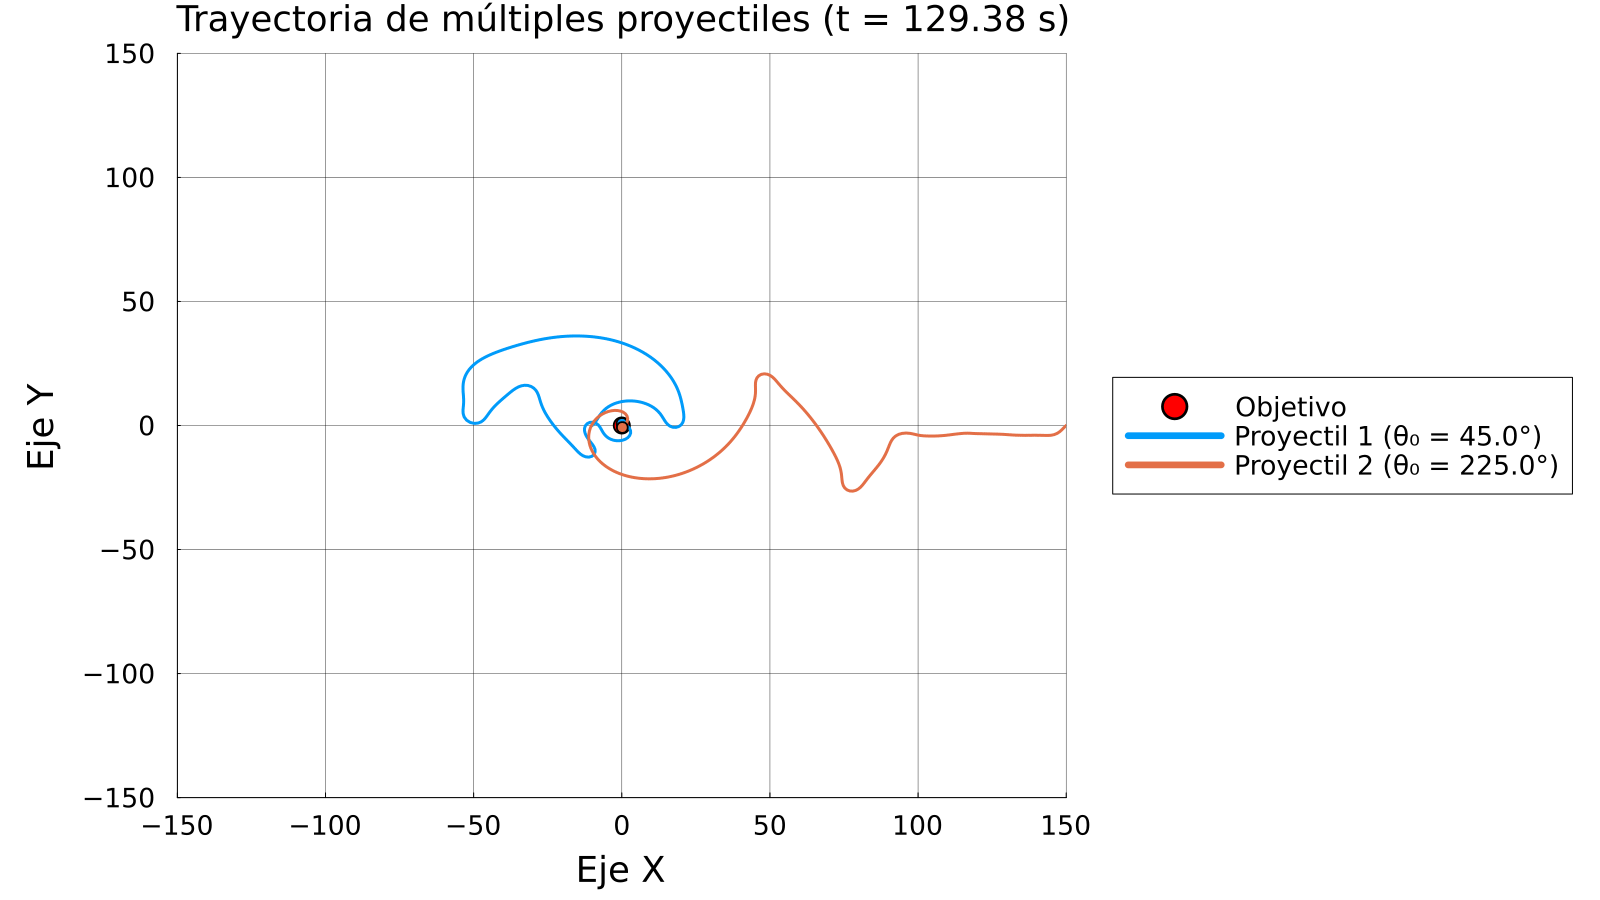
\includegraphics[width=\linewidth]{multiproyectil/posiciones_lejanas_gamma_0.0001_final.png}
  \caption{Último fotograma de la animación guardada con $\gamma=0.0001$. \href{run:figuras/multiproyectil/posiciones_lejanas_gamma_0.0001.gif}{Animación original}.}
  \label{fig:multi-lejanas-baja}
\end{figure}


\clearpage
\nocite{*}
\bibliography{library}
